% !TEX program = pdflatex
% !TEX options = -synctex=1 -interaction=nonstopmode -file-line-error "%DOC%"
% Nonlinear Optics Assignment 6
\documentclass[UTF8,10pt,a4paper]{article}
\usepackage[scheme=plain]{ctex}
\newcommand{\CourseName}{Nonlinear Optics}
\newcommand{\CourseCode}{PHYS2202}
\newcommand{\Semester}{Spring, 2020}
\newcommand{\ProjectName}{Assignment 6}
\newcommand{\DueTimeType}{Due Time}
\newcommand{\DueTime}{17:00, May 14, 2020 (Thursday)}
\newcommand{\StudentName}{陈稼霖}
\newcommand{\StudentID}{45875852}
\usepackage[vmargin=1in,hmargin=.5in]{geometry}
\usepackage{fancyhdr}
\usepackage{lastpage}
\usepackage{calc}
\pagestyle{fancy}
\fancyhf{}
\fancyhead[L]{\CourseName}
\fancyhead[C]{\ProjectName}
\fancyhead[R]{\StudentName}
\fancyfoot[R]{\thepage\ / \pageref{LastPage}}
\setlength\headheight{12pt}
\fancypagestyle{FirstPageStyle}{
    \fancyhf{}
    \fancyhead[L]{\CourseName\\
        \CourseCode\\
        \Semester}
    \fancyhead[C]{{\Huge\bfseries\ProjectName}\\
        \DueTimeType\ : \DueTime}
    \fancyhead[R]{Name : \makebox[\widthof{\StudentID}][s]{\StudentName}\\
        Student ID\@ : \StudentID\\
        Score : \underline{\makebox[\widthof{\StudentID}]{}}}
    \fancyfoot[R]{\thepage\ / \pageref{LastPage}}
    \setlength\headheight{36pt}
}
\usepackage{amsmath,amssymb,amsthm,bm}
\allowdisplaybreaks[4]
\newtheoremstyle{Problem}
{}
{}
{}
{}
{\bfseries}
{.}
{ }
{\thmname{#1}\thmnumber{ #2}\thmnote{ (#3)} Score: \underline{\qquad\qquad}}
\theoremstyle{Problem}
\newtheorem{prob}{Problem}
\newtheoremstyle{Solution}
{}
{}
{}
{}
{\bfseries}
{:}
{ }
{\thmname{#1}}
\makeatletter
\def\@endtheorem{\qed\endtrivlist\@endpefalse}
\makeatother
\theoremstyle{Solution}
\newtheorem*{sol}{Solution}
\usepackage{ulem}
\usepackage{graphicx}
% \usepackage{multirow}
\begin{document}
\thispagestyle{FirstPageStyle}
\begin{prob}[(20 points)]
    \textbf{Context:} Except for the final equation, the contextual information is not needed to solve the problem; it is just to explain why we would consider such a problem.\\
    Throughout the course, we have used the electric-dipole approximation. Namely, we have assumed that the interaction Hamiltonian between the optical fields and the medium is give by
    \begin{align}
        \hat{H}_I=\hat{H}_{ED}=-\sum_jq_j\hat{\vec{r}}_j\cdot\vec{E}(\vec{r}_j),
    \end{align}
    where $q_j$ is the charge of particle $j$ located at position $\vec{r}_j$. This approximation is reasonable since the wavelengths of optical field are long compared to the size of an atom, molecule, or crystal lattice period. We have seen, though, that for a crystal of given symmetry, there are certain combinations of input and output electric field polarizations for which the $n^{\text{th}}$ order nonlinear response \textit{in the electric-dipole approximation} (ED) is zero because $\hat{u}\cdot\overleftrightarrow{\chi}_{\text{ED}}:\hat{a}\hat{b}\cdots\hat{n}=\chi_{\text{ED},uab\ldots n}=0$. For such combinations of polarizations, we might still see a non-zero $n^{\text{th}}$ order nonlinear optical response (i.e., a response that depends on $n$ interactions with the electric field), but this response will be due to typically weak but non-zero non-dipolar contributions.\\
    The leading order non-dipolar contributions to the optical response of a material are typically the electric quadrupole response and the magnetic dipole response. Let us consider the electric quadrupole response. Our elementary model for a electric quadrupole is two oppositely aligned electric dipoles of equal magnitude next to one another. To \textit{induce} an electric quadrupole, the electric field cannot be constant across the material; the electric field must be spatially varying on a short enough time scale to push like charges in opposite direction. We can write the quadrupolar interaction Hamiltonian as
    \begin{align}
        \hat{H}_{EQ}=-\frac{1}{6}\sum_{i,j}Q_{i,j}\frac{\partial}{\partial x_i}\vec{E}_j(\vec{r}),
    \end{align}
    where the "molecular" (here we use the term in an extended sense to mean a microscopic object: atom, molecule, or unit cell) quadrupole operator $\overleftrightarrow{Q}$ for a collection of point charges is
    \begin{align}
        \overleftrightarrow{Q}_{ij}=\frac{1}{6}\sum_n(3x_{n,i}x_{n,j}-r^2\delta_{ij})q_n
    \end{align}
    Just as we saw that we can express the dipolar response in terms of a \textit{local} susceptibility $\overleftrightarrow{\chi}^{(n)}$, the \textit{nonlocal} electric quadrupole response (nonlocal because the response depends on the fact that the electric field has a spatial variation; there is a difference in electric field between two locations) can be expressed in terms of an $n^{\text{th}}$ order nonlocal susceptibility $\overleftrightarrow{\chi}_{EQ}^{(n)}$. For example, the second-order electric quadrupole response can be written
    \begin{align}
        P_u^{(2)}(\omega)=\sum_{a,b,c}\chi_{\text{EQ},uabc}^{(2)}(-\omega;\omega_1,\omega_2)E_a(\omega_1)\frac{d}{dx_b}E_c(\omega_2).
    \end{align}
    Note that the $n^{\text{th}}$ order electric quadrupole contribution to the susceptibility is characterized by four indices instead of the three indices characterizing the dipolar $\overleftrightarrow{\chi}^{(2)}$, so although they are both labeled here by a $(2)$ superscript they tensors are not the same rank.\\
    \textbf{Question:} Consider the $3m$ crystal class whose stereogram is illustrated below. The filled circles represent atoms above the plane of the page. The only symmetry operation of this system are the three-fold rotation about the $z$ axis (out of the page), i.e., rotation of $2\pi/3$ and $4\pi/3$, and a mirror plane perpendicular to the $x$ axis (in the $yz$ plane). Note that the three-fold symmetry means that there must be three mirror reflection planes. Find all combinations of input and output polarizations that could yield a non-zero polarization; that is find all the non-zero quadrupole susceptibility elements $\chi_{\text{EQ},ijkl}^{(2)}$. Identify the dependencies between elements that are not independent.\\
    Note: You must demonstrate which elements are potentially non-zero and their dependencies. You can not just give the result.
    \begin{figure}[h]
        \centering
        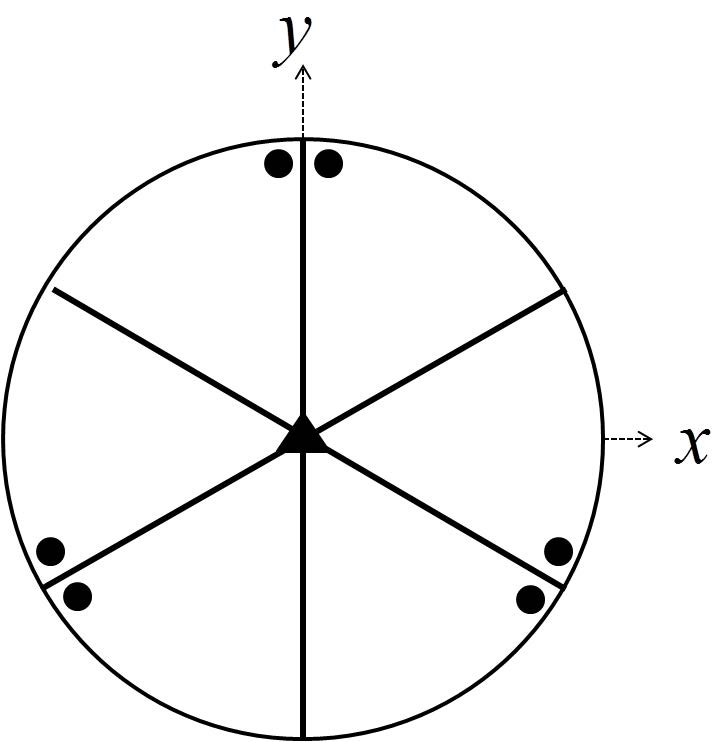
\includegraphics[width=.16\textwidth]{stereogram-3m.jpg}
    \end{figure}
\end{prob}
\begin{sol}
    Zero polarization means that both the dipolar polarization and the quadrupolar polarization are zero, and non-zero polarization means that at least one of the zero polarization and the quadrupolar polarization is non-zero, so we need discuss both dipolar and quadrupolar polarization to find the combinations of input and output directions that produce non-zero polarization.
    \section{$2$nd order Electric dipolar polarization}
    The $2$nd order electric polarization is
    \begin{align}
        \vec{P}_{\text{EQ}}^{(2)}(\omega)=\overleftrightarrow{\chi}_{\text{ED}}^{(2)}(-\omega;\omega_1,\omega_2):\vec{E}(\omega_1)\vec{E}(\omega_2).
    \end{align}
    The component form of the above equation is
    \begin{align}
        P_{\text{ED},u}^{(2)}(\omega)=\chi_{\text{EQ},uab}^{(2)}(-\omega;\omega_1,\omega_2)E_a(\omega_1)E_b(\omega_2).
    \end{align}
    Note that we are using the Einstein summation convention (repeated indices implies summation over this indices).
    Rotating the system by some angle about some axis is equivalent to rotating the input field and the output polarization in the opposite sense with the system unchanged. In this way, after the rotation the polarization should be
    \begin{align}
        \vec{P}_{\text{EQ},u}^{'(2)}=\overleftrightarrow{\chi}_{\text{ED}}^{(2)}(-\omega;\omega_1,\omega_2):\vec{E}(\omega_1)E(\omega_2).
    \end{align}
    The component form of the above equation is
    \begin{align}
        \label{P-ED-1}
        P_{\text{EQ},\mu}^{'(2)}(\omega)=\chi_{\text{EQ},\mu\alpha\beta}E_{\alpha}(\omega_1)E_{\beta}(\omega_2).
    \end{align}
    From another perspective, we can also just rotate only the system and thus the susceptibility, so
    \begin{align}
        \vec{P}_{\text{ED}}^{(2)}=[\hat{R}\overleftrightarrow{\chi}^{(2)}]:\vec{E}(\omega_1)\vec{E}(\omega_2),
    \end{align}
    where $\hat{R}$ is the representation matrix of the rotation operation.
    The component form of the above equation is
    \begin{align}
        P_{\text{ED},\mu}^{'(2)}=R_{\mu u}\chi_{\text{ED},uab}^{(2)}E_a(\omega_1)E_b(\omega_2).
    \end{align}
    Note that the vector $\vec{v}$ before the rotation is just given by multiplying the vector $\vec{v}'$ after the rotation with the representation matrix of the rotation operator, so we have
    \begin{align}
        \label{P_ED-2}
        P_{\text{ED},\mu}^{'(2)}=R_{\mu u}\chi_{\text{ED},uab}^{(2)}E_a(\omega_1)E_b(\omega_2)=R_{\mu u}\chi_{\text{ED},uab}^{(2)}R_{\alpha a}E_{\alpha}'(\omega_1)R_{\beta b}E_{\beta}'(\omega_2)=R_{\mu u}R_{\alpha a}R_{\beta b}\chi_{\text{ED},uab}^{(2)}E_{\alpha}'(\omega_1)E_{\beta}'(\omega_2).
    \end{align}
    Comparing equation and equation, we get
    \begin{align}
        \chi_{\text{ED},\mu\alpha\beta}^{(2)}=R_{\mu u}R_{\alpha a}R_{\beta b}\chi_{\text{ED},uab}^{(2)}
    \end{align}




    \subsection{Information derived from $m_{100}$}
    Suppose we reflect the system by the mirror plane perpendicular to $(1,0,0)$. This operation can be represented by the matrix:
    \begin{align}
        R(m_{100})=\left(\begin{matrix}
            -1&0&0\\
            0&1&0\\
            0&0&1
        \end{matrix}\right).
    \end{align}
    After the reflection, the $2$nd order electric dipolar susceptibility must satisfy
    \begin{align}
        \nonumber\chi_{\text{ED},\mu\alpha\beta}^{(2)}=&R_{\mu u}(m_{100})R_{\alpha a}(m_{100})R_{\beta b}(m_{100})\chi_{EQ,uab}\\
        =&[\delta_{\mu x}+\delta_{\mu y}+\delta_{\mu z}][-\delta_{\alpha x}+\delta_{\alpha y}+\delta_{\alpha z}][-\delta_{\beta x}+\delta_{\beta y}+\delta_{\beta z}]\chi_{\text{ED},\mu\alpha\beta}.
    \end{align}
    According to the above equation, there are two kinds of cases:
    \begin{itemize}
        \item In \textbf{cases that the number of $x$ in $\{\mu,\alpha,\beta\}$ is odd}, we have
        \begin{align}
            \chi_{\text{ED},\mu\alpha\beta}^{(2)}=-\chi_{\text{ED},\mu\alpha\beta}^{(2)},
        \end{align}
        so
        \begin{align}
            \chi_{\text{ED},\mu\alpha\beta}^{(2)}=0.
        \end{align}
        \item In \textbf{cases that the number of $x$ in $\{\mu,\alpha,\beta\}$ is even}, we have
        \begin{align}
            \chi_{\text{ED},\mu\alpha\beta}^{(2)}=\chi_{\text{ED},\mu\alpha\beta}^{(2)}.
        \end{align}
        This trivial equation can not provide any useful information for us.
    \end{itemize}
    % Therefore, $\chi_{\text{ED},\mu\alpha\beta}$ is non-zero only if there are zero or two $x$ in $\{\mu,\alpha,\beta\}$. The non-zero $\chi_{\text{ED},\mu\alpha\beta}$ are
    % \begin{gather*}
    %     \chi_{\text{ED},yyy},\quad\chi_{\text{ED},yyz},\quad\chi_{\text{ED},yzy},\quad\chi_{\text{ED},yzz},\quad\chi_{\text{ED},zyy},\quad\chi_{\text{ED},zyz},\quad\chi_{\text{ED},zzy},\quad\chi_{\text{ED},zzz},\\
    %     \chi_{\text{ED},xxy},\quad\chi_{\text{ED},xxz},\quad\chi_{\text{ED},yxx},\quad\chi_{\text{ED},zxx},\quad\chi_{\text{ED},xyx},\quad\chi_{\text{ED},xzx}.
    % \end{gather*}
    The $\chi_{\text{ED},\mu\alpha\beta}^{(2)}$ required by the symmetry operation $m_{100}$ to be zero are
    \small
    \begin{gather*}
        \chi_{\text{ED},xyy}^{(2)},\quad\chi_{\text{ED},xyz}^{(2)},\quad\chi_{\text{ED},xzy}^{(2)},\quad\chi_{\text{ED},xzz}^{(2)},\quad\chi_{\text{ED},yxy}^{(2)},\quad\chi_{\text{ED},yxz}^{(2)},\quad\chi_{\text{ED},zxy}^{(2)},\quad\chi_{\text{ED},zxz}^{(2)},\quad\chi_{\text{ED},yyx}^{(2)},\quad\chi_{\text{ED},yzx}^{(2)},\quad\chi_{\text{ED},zyx}^{(2)},\quad\chi_{\text{ED},zzx}^{(2)},\\
        \chi_{\text{ED},xxx}^{(2)}.
    \end{gather*}
    \normalsize



    \subsection{Information derived from $3_z$}
    Suppose we rotate the system by $\frac{2\pi}{3}$ about the $z$ axis counterclockwisely. This rotation can represented by the matrix:
    \begin{align}
        R(3_z)=\left(\begin{matrix}
            \cos\frac{2\pi}{3}&-\sin\frac{2\pi}{3}&0\\
            \sin\frac{2\pi}{3}&\cos\frac{2\pi}{3}&0\\
            0&0&1
        \end{matrix}\right)=\left(\begin{matrix}
            \frac{1}{2}&-\frac{\sqrt{3}}{2}&0\\
            \frac{\sqrt{3}}{2}&\frac{1}{2}&0\\
            0&0&1
        \end{matrix}\right).
    \end{align}
    Under this rotation, the $2$nd order electric quadrupolar susceptibility must satisfy
    \begin{align}
        \chi_{\text{ED},\mu\alpha\beta}^{(2)}=R_{\mu u}(3_z)R_{\alpha a}(3_z)R_{\beta b}(3_z)\chi_{\text{ED},uab}^{(2)}.
    \end{align}
    Since $\chi_{\text{ED},\mu\alpha\beta}$ is non-zero only if there are zero or two $x$ in $\{\mu,\alpha,\beta\}$,
    \small
    \begin{align}
        \nonumber\chi_{\text{ED},\mu\alpha\beta}^{(2)}=&\sum_{u\in\{y,z\}}\sum_{a\in\{y,z\}}\sum_{b\in\{y,z\}}R_{\mu u}(3_z)R_{\alpha a}(3_z)R_{\beta b}(3_z)\chi_{\text{ED},uab}^{(2)}\\
        &+\sum_{b\in\{y,z\}}R_{\mu x}(3_z)R_{\alpha x}(3_z)R_{\beta b}(3_z)\chi_{\text{ED},xx\beta}^{(2)}+\sum_{u\in\{y,z\}}R_{\mu u}(3_z)R_{\alpha x}(3_z)R_{\beta x}(3_z)\chi_{\text{ED},uxx}^{(2)}+\sum_{a\in\{y,z\}}R_{\mu x}(3_z)R_{\alpha a}(3_z)R_{\beta x}(3_z)\chi_{\text{ED},xax}^{(2)}.
    \end{align}
    \normalsize

    The above equation can give $27$ relations of the $2$nd order electric dipolar susceptibility:
\begin{itemize}
\item For $u=x,\alpha=x,\beta=x$, we have
\small\begin{align}
\nonumber\chi_{\text{ED},xxx}^{(2)}=&\left(-\frac{\sqrt{3}}{2}\right)\left(-\frac{\sqrt{3}}{2}\right)\left(-\frac{\sqrt{3}}{2}\right)\chi_{\text{ED},yyy}^{(2)}\\
&+\left[\left(-\frac{1}{2}\right)\left(-\frac{1}{2}\right)\left(-\frac{\sqrt{3}}{2}\right)\chi_{\text{ED},xxy}^{(2)}\right]+\left[\left(-\frac{\sqrt{3}}{2}\right)\left(-\frac{1}{2}\right)\left(-\frac{1}{2}\right)\chi_{\text{ED},yxx}^{(2)}\right]+\left[\left(-\frac{1}{2}\right)\left(-\frac{\sqrt{3}}{2}\right)\left(-\frac{1}{2}\right)\chi_{\text{ED},xyx}^{(2)}\right]
\end{align}\normalsize
\item For $u=x,\alpha=x,\beta=y$, we have
\small\begin{align}
\nonumber\chi_{\text{ED},xxy}^{(2)}=&\left(-\frac{\sqrt{3}}{2}\right)\left(-\frac{\sqrt{3}}{2}\right)\left(-\frac{1}{2}\right)\chi_{\text{ED},yyy}^{(2)}\\
&+\left[\left(-\frac{1}{2}\right)\left(-\frac{1}{2}\right)\left(-\frac{1}{2}\right)\chi_{\text{ED},xxy}^{(2)}\right]+\left[\left(-\frac{\sqrt{3}}{2}\right)\left(-\frac{1}{2}\right)\frac{\sqrt{3}}{2}\chi_{\text{ED},yxx}^{(2)}\right]+\left[\left(-\frac{1}{2}\right)\left(-\frac{\sqrt{3}}{2}\right)\frac{\sqrt{3}}{2}\chi_{\text{ED},xyx}^{(2)}\right]
\end{align}\normalsize
\item For $u=x,\alpha=x,\beta=z$, we have
\small\begin{align}
\nonumber\chi_{\text{ED},xxz}^{(2)}=&\left(-\frac{\sqrt{3}}{2}\right)\left(-\frac{\sqrt{3}}{2}\right)1\chi_{\text{ED},yyz}^{(2)}\\
&+\left[\left(-\frac{1}{2}\right)\left(-\frac{1}{2}\right)1\chi_{\text{ED},xxz}^{(2)}\right]
\end{align}\normalsize
\item For $u=x,\alpha=y,\beta=x$, we have
\small\begin{align}
\nonumber\chi_{\text{ED},xyx}^{(2)}=&\left(-\frac{\sqrt{3}}{2}\right)\left(-\frac{1}{2}\right)\left(-\frac{\sqrt{3}}{2}\right)\chi_{\text{ED},yyy}^{(2)}\\
&+\left[\left(-\frac{1}{2}\right)\frac{\sqrt{3}}{2}\left(-\frac{\sqrt{3}}{2}\right)\chi_{\text{ED},xxy}^{(2)}\right]+\left[\left(-\frac{\sqrt{3}}{2}\right)\frac{\sqrt{3}}{2}\left(-\frac{1}{2}\right)\chi_{\text{ED},yxx}^{(2)}\right]+\left[\left(-\frac{1}{2}\right)\left(-\frac{1}{2}\right)\left(-\frac{1}{2}\right)\chi_{\text{ED},xyx}^{(2)}\right]
\end{align}\normalsize
\item For $u=x,\alpha=y,\beta=y$, we have
\small\begin{align}
\nonumber\chi_{\text{ED},xyy}^{(2)}=&\left(-\frac{\sqrt{3}}{2}\right)\left(-\frac{1}{2}\right)\left(-\frac{1}{2}\right)\chi_{\text{ED},yyy}^{(2)}\\
&+\left[\left(-\frac{1}{2}\right)\frac{\sqrt{3}}{2}\left(-\frac{1}{2}\right)\chi_{\text{ED},xxy}^{(2)}\right]+\left[\left(-\frac{\sqrt{3}}{2}\right)\frac{\sqrt{3}}{2}\frac{\sqrt{3}}{2}\chi_{\text{ED},yxx}^{(2)}\right]+\left[\left(-\frac{1}{2}\right)\left(-\frac{1}{2}\right)\frac{\sqrt{3}}{2}\chi_{\text{ED},xyx}^{(2)}\right]
\end{align}\normalsize
\item For $u=x,\alpha=y,\beta=z$, we have
\small\begin{align}
\nonumber\chi_{\text{ED},xyz}^{(2)}=&\left(-\frac{\sqrt{3}}{2}\right)\left(-\frac{1}{2}\right)1\chi_{\text{ED},yyz}^{(2)}\\
&+\left[\left(-\frac{1}{2}\right)\frac{\sqrt{3}}{2}1\chi_{\text{ED},xxz}^{(2)}\right]
\end{align}\normalsize
\item For $u=x,\alpha=z,\beta=x$, we have
\small\begin{align}
\nonumber\chi_{\text{ED},xzx}^{(2)}=&\left(-\frac{\sqrt{3}}{2}\right)1\left(-\frac{\sqrt{3}}{2}\right)\chi_{\text{ED},yzy}^{(2)}\\
&+\left[\left(-\frac{1}{2}\right)1\left(-\frac{1}{2}\right)\chi_{\text{ED},xzx}^{(2)}\right]
\end{align}\normalsize
\item For $u=x,\alpha=z,\beta=y$, we have
\small\begin{align}
\nonumber\chi_{\text{ED},xzy}^{(2)}=&\left(-\frac{\sqrt{3}}{2}\right)1\left(-\frac{1}{2}\right)\chi_{\text{ED},yzy}^{(2)}\\
&+\left[\left(-\frac{1}{2}\right)1\frac{\sqrt{3}}{2}\chi_{\text{ED},xzx}^{(2)}\right]
\end{align}\normalsize
\item For $u=x,\alpha=z,\beta=z$, we have
\small\begin{align}
\nonumber\chi_{\text{ED},xzz}^{(2)}=&\left(-\frac{\sqrt{3}}{2}\right)11\chi_{\text{ED},yzz}^{(2)}\\
&
\end{align}\normalsize
\item For $u=y,\alpha=x,\beta=x$, we have
\small\begin{align}
\nonumber\chi_{\text{ED},yxx}^{(2)}=&\left(-\frac{1}{2}\right)\left(-\frac{\sqrt{3}}{2}\right)\left(-\frac{\sqrt{3}}{2}\right)\chi_{\text{ED},yyy}^{(2)}\\
&+\left[\frac{\sqrt{3}}{2}\left(-\frac{1}{2}\right)\left(-\frac{\sqrt{3}}{2}\right)\chi_{\text{ED},xxy}^{(2)}\right]+\left[\left(-\frac{1}{2}\right)\left(-\frac{1}{2}\right)\left(-\frac{1}{2}\right)\chi_{\text{ED},yxx}^{(2)}\right]+\left[\frac{\sqrt{3}}{2}\left(-\frac{\sqrt{3}}{2}\right)\left(-\frac{1}{2}\right)\chi_{\text{ED},xyx}^{(2)}\right]
\end{align}\normalsize
\item For $u=y,\alpha=x,\beta=y$, we have
\small\begin{align}
\nonumber\chi_{\text{ED},yxy}^{(2)}=&\left(-\frac{1}{2}\right)\left(-\frac{\sqrt{3}}{2}\right)\left(-\frac{1}{2}\right)\chi_{\text{ED},yyy}^{(2)}\\
&+\left[\frac{\sqrt{3}}{2}\left(-\frac{1}{2}\right)\left(-\frac{1}{2}\right)\chi_{\text{ED},xxy}^{(2)}\right]+\left[\left(-\frac{1}{2}\right)\left(-\frac{1}{2}\right)\frac{\sqrt{3}}{2}\chi_{\text{ED},yxx}^{(2)}\right]+\left[\frac{\sqrt{3}}{2}\left(-\frac{\sqrt{3}}{2}\right)\frac{\sqrt{3}}{2}\chi_{\text{ED},xyx}^{(2)}\right]
\end{align}\normalsize
\item For $u=y,\alpha=x,\beta=z$, we have
\small\begin{align}
\nonumber\chi_{\text{ED},yxz}^{(2)}=&\left(-\frac{1}{2}\right)\left(-\frac{\sqrt{3}}{2}\right)1\chi_{\text{ED},yyz}^{(2)}\\
&+\left[\frac{\sqrt{3}}{2}\left(-\frac{1}{2}\right)1\chi_{\text{ED},xxz}^{(2)}\right]
\end{align}\normalsize
\item For $u=y,\alpha=y,\beta=x$, we have
\small\begin{align}
\nonumber\chi_{\text{ED},yyx}^{(2)}=&\left(-\frac{1}{2}\right)\left(-\frac{1}{2}\right)\left(-\frac{\sqrt{3}}{2}\right)\chi_{\text{ED},yyy}^{(2)}\\
&+\left[\frac{\sqrt{3}}{2}\frac{\sqrt{3}}{2}\left(-\frac{\sqrt{3}}{2}\right)\chi_{\text{ED},xxy}^{(2)}\right]+\left[\left(-\frac{1}{2}\right)\frac{\sqrt{3}}{2}\left(-\frac{1}{2}\right)\chi_{\text{ED},yxx}^{(2)}\right]+\left[\frac{\sqrt{3}}{2}\left(-\frac{1}{2}\right)\left(-\frac{1}{2}\right)\chi_{\text{ED},xyx}^{(2)}\right]
\end{align}\normalsize
\item For $u=y,\alpha=y,\beta=y$, we have
\small\begin{align}
\nonumber\chi_{\text{ED},yyy}^{(2)}=&\left(-\frac{1}{2}\right)\left(-\frac{1}{2}\right)\left(-\frac{1}{2}\right)\chi_{\text{ED},yyy}^{(2)}\\
&+\left[\frac{\sqrt{3}}{2}\frac{\sqrt{3}}{2}\left(-\frac{1}{2}\right)\chi_{\text{ED},xxy}^{(2)}\right]+\left[\left(-\frac{1}{2}\right)\frac{\sqrt{3}}{2}\frac{\sqrt{3}}{2}\chi_{\text{ED},yxx}^{(2)}\right]+\left[\frac{\sqrt{3}}{2}\left(-\frac{1}{2}\right)\frac{\sqrt{3}}{2}\chi_{\text{ED},xyx}^{(2)}\right]
\end{align}\normalsize
\item For $u=y,\alpha=y,\beta=z$, we have
\small\begin{align}
\nonumber\chi_{\text{ED},yyz}^{(2)}=&\left(-\frac{1}{2}\right)\left(-\frac{1}{2}\right)1\chi_{\text{ED},yyz}^{(2)}\\
&+\left[\frac{\sqrt{3}}{2}\frac{\sqrt{3}}{2}1\chi_{\text{ED},xxz}^{(2)}\right]
\end{align}\normalsize
\item For $u=y,\alpha=z,\beta=x$, we have
\small\begin{align}
\nonumber\chi_{\text{ED},yzx}^{(2)}=&\left(-\frac{1}{2}\right)1\left(-\frac{\sqrt{3}}{2}\right)\chi_{\text{ED},yzy}^{(2)}\\
&+\left[\frac{\sqrt{3}}{2}1\left(-\frac{1}{2}\right)\chi_{\text{ED},xzx}^{(2)}\right]
\end{align}\normalsize
\item For $u=y,\alpha=z,\beta=y$, we have
\small\begin{align}
\nonumber\chi_{\text{ED},yzy}^{(2)}=&\left(-\frac{1}{2}\right)1\left(-\frac{1}{2}\right)\chi_{\text{ED},yzy}^{(2)}\\
&+\left[\frac{\sqrt{3}}{2}1\frac{\sqrt{3}}{2}\chi_{\text{ED},xzx}^{(2)}\right]
\end{align}\normalsize
\item For $u=y,\alpha=z,\beta=z$, we have
\small\begin{align}
\nonumber\chi_{\text{ED},yzz}^{(2)}=&\left(-\frac{1}{2}\right)11\chi_{\text{ED},yzz}^{(2)}\\
&
\end{align}\normalsize
which means that
\begin{align}
    \chi_{\text{ED},yzz}^{(2)}=0,
\end{align}
and thus
\begin{align}
    \chi_{\text{ED},xzz}^{(2)}=0.
\end{align}
\item For $u=z,\alpha=x,\beta=x$, we have
\small\begin{align}
\nonumber\chi_{\text{ED},zxx}^{(2)}=&1\left(-\frac{\sqrt{3}}{2}\right)\left(-\frac{\sqrt{3}}{2}\right)\chi_{\text{ED},zyy}^{(2)}\\
&+\left[1\left(-\frac{1}{2}\right)\left(-\frac{1}{2}\right)\chi_{\text{ED},zxx}^{(2)}\right]
\end{align}\normalsize
\item For $u=z,\alpha=x,\beta=y$, we have
\small\begin{align}
\nonumber\chi_{\text{ED},zxy}^{(2)}=&1\left(-\frac{\sqrt{3}}{2}\right)\left(-\frac{1}{2}\right)\chi_{\text{ED},zyy}^{(2)}\\
&+\left[1\left(-\frac{1}{2}\right)\frac{\sqrt{3}}{2}\chi_{\text{ED},zxx}^{(2)}\right]
\end{align}\normalsize
\item For $u=z,\alpha=x,\beta=z$, we have
\small\begin{align}
\nonumber\chi_{\text{ED},zxz}^{(2)}=&1\left(-\frac{\sqrt{3}}{2}\right)1\chi_{\text{ED},zyz}^{(2)}\\
&
\end{align}\normalsize
\item For $u=z,\alpha=y,\beta=x$, we have
\small\begin{align}
\nonumber\chi_{\text{ED},zyx}^{(2)}=&1\left(-\frac{1}{2}\right)\left(-\frac{\sqrt{3}}{2}\right)\chi_{\text{ED},zyy}^{(2)}\\
&+\left[1\frac{\sqrt{3}}{2}\left(-\frac{1}{2}\right)\chi_{\text{ED},zxx}^{(2)}\right]
\end{align}\normalsize
\item For $u=z,\alpha=y,\beta=y$, we have
\small\begin{align}
\nonumber\chi_{\text{ED},zyy}^{(2)}=&1\left(-\frac{1}{2}\right)\left(-\frac{1}{2}\right)\chi_{\text{ED},zyy}^{(2)}\\
&+\left[1\frac{\sqrt{3}}{2}\frac{\sqrt{3}}{2}\chi_{\text{ED},zxx}^{(2)}\right]
\end{align}\normalsize
\item For $u=z,\alpha=y,\beta=z$, we have
\small\begin{align}
\nonumber\chi_{\text{ED},zyz}^{(2)}=&1\left(-\frac{1}{2}\right)1\chi_{\text{ED},zyz}^{(2)}\\
&
\end{align}\normalsize
which means that
\begin{align}
    \chi_{\text{ED},zyz}^{(2)}=0,
\end{align}
and thus
\begin{align}
    \chi_{\text{ED},zxz}^{(2)}=0.
\end{align}
\item For $u=z,\alpha=z,\beta=x$, we have
\small\begin{align}
\nonumber\chi_{\text{ED},zzx}^{(2)}=&11\left(-\frac{\sqrt{3}}{2}\right)\chi_{\text{ED},zzy}^{(2)}\\
&
\end{align}\normalsize
\item For $u=z,\alpha=z,\beta=y$, we have
\small\begin{align}
\nonumber\chi_{\text{ED},zzy}^{(2)}=&11\left(-\frac{1}{2}\right)\chi_{\text{ED},zzy}^{(2)}\\
&
\end{align}\normalsize
which means that
\begin{align}
    \chi_{\text{ED},zzy}^{(2)}=0,
\end{align}
and thus
\begin{align}
    \chi_{\text{ED},zzx}^{(2)}=0.
\end{align}
\item For $u=z,\alpha=z,\beta=z$, we have
\small\begin{align}
\nonumber\chi_{\text{ED},zzz}^{(2)}=&111\chi_{\text{ED},zzz}^{(2)}\\
&
\end{align}\normalsize
\end{itemize}

    The $\chi_{\text{ED},\mu\alpha\beta}$ required by the symmetry operation $C_z$ to be zero are
    \begin{gather*}
        \chi_{\text{ED},yzz}^{(2)},\quad\chi_{\text{ED},zyz}^{(2)},\quad\chi_{\text{ED},zzy}^{(2)}.
    \end{gather*}

    Now we discussed the information derived from the rotation $3_z$ and the reflection $m_{100}$, the discussion about $(3_z)^2,m_{1,\sqrt{3},0},m_{1,-\sqrt{3},0}$ is not needed, because these operation are combinations of $3_z$ and $m_{100}$
    \begin{align}
        (3_z)^2=&3_z\times 3_z,\\
        m_{1,\sqrt{3},0}=&3_z\times m_{100},\\
        m_{1,-\sqrt{3},0}=&3_z\times 3_z\times m_{100},
    \end{align}
    if the polarization do not change after operation $A$ and operation $B$ respectively, it will not change after applying operation $A$ then followed by operation $B$.

    Therefore, all the $\chi_{\text{ED},\mu\alpha\beta}$ required to be zero are ($16$ elements in total)
    \small
    \begin{gather*}
        \chi_{\text{ED},xyy}^{(2)},\quad\chi_{\text{ED},xyz}^{(2)},\quad\chi_{\text{ED},xzy}^{(2)},\quad\chi_{\text{ED},xzz}^{(2)},\quad\chi_{\text{ED},yxy}^{(2)},\quad\chi_{\text{ED},yxz}^{(2)},\quad\chi_{\text{ED},zxy}^{(2)},\quad\chi_{\text{ED},zxz}^{(2)},\quad\chi_{\text{ED},yyx}^{(2)},\quad\chi_{\text{ED},yzx}^{(2)},\quad\chi_{\text{ED},zyx}^{(2)},\quad\chi_{\text{ED},zzx}^{(2)},\\
        \chi_{\text{ED},xxx}^{(2)},\\
        \chi_{\text{ED},yzz}^{(2)},\quad\chi_{\text{ED},zyz}^{(2)},\quad\chi_{\text{ED},zzy}^{(2)}.
    \end{gather*}
    \normalsize
    All the none-zero $\chi_{\text{ED},\mu\alpha\beta}^{(2)}$ are ($11$ elements in total)
    \begin{gather*}
        \chi_{\text{ED},yyy}^{(2)},\quad\chi_{\text{ED},yyz}^{(2)},\quad\chi_{\text{ED},yzy}^{(2)},\quad\chi_{\text{ED},zyy}^{(2)},\quad\chi_{\text{ED},zzz}^{(2)},\\
        \chi_{\text{ED},xxy}^{(2)},\quad,\chi_{\text{ED},xxz}^{(2)}\quad\chi_{\text{ED},yxx}^{(2)},\quad\chi_{\text{ED},zxx}^{(2)},\quad\chi_{\text{ED},xyx},\quad\chi_{\text{ED},xzx}^{(2)}.
    \end{gather*}
    \uline{If we only consider dipole contribution to the polarization}, the combinations of input and output polarizations that could yield a \uline{non-zero} polarization are shown in table \ref{ED-NZ} and the combinations that could yield a \uline{zero} polarization zre shown in table \ref{ED-Z}.
    \begin{table}[h]
        \centering
        \caption{The combinations of input and output polarization that could yield a \uline{non-zero} polarization (\uline{if only considering dipole contribution to the polarization}) ($11$ combinations in total).}
        \label{ED-NZ}
        \begin{tabular}{|c|c|c|}
        \hline
        \begin{tabular}[c]{@{}c@{}}The direction of $\vec{P}$\\ (along which axis)\end{tabular} & \begin{tabular}[c]{@{}c@{}}The driction of $\vec{E}(\omega_1)$\\ (along which axis)\end{tabular} & \begin{tabular}[c]{@{}c@{}}The direction of $\vec{E}(\omega_2)$\\ (along which axis)\end{tabular} \\ \hline
        $y$ & $y$ & $y$ \\ \hline
        $y$ & $y$ & $z$ \\ \hline
        $y$ & $z$ & $y$ \\ \hline
        $z$ & $y$ & $y$ \\ \hline
        $z$ & $z$ & $z$ \\ \hline
        $x$ & $x$ & $y$ \\ \hline
        $x$ & $x$ & $z$ \\ \hline
        $y$ & $x$ & $x$ \\ \hline
        $z$ & $x$ & $x$ \\ \hline
        $x$ & $y$ & $x$ \\ \hline
        $x$ & $z$ & $x$ \\ \hline
        \end{tabular}
    \end{table}
    \begin{table}[h]
        \centering
        \caption{The combinations of input and output polarization that could yield a \uline{zero} polarization (\uline{if only considering dipole contribution to the polarization}) ($16$ combinations in total).}
        \label{ED-Z}
        \begin{tabular}{|c|c|c|}
        \hline
        \begin{tabular}[c]{@{}c@{}}The direction of $\vec{P}$\\ (along which axis)\end{tabular} & \begin{tabular}[c]{@{}c@{}}The driction of $\vec{E}(\omega_1)$\\ (along which axis)\end{tabular} & \begin{tabular}[c]{@{}c@{}}The direction of $\vec{E}(\omega_2)$\\ (along which axis)\end{tabular} \\ \hline
        $x$ & $y$ & $y$ \\ \hline
        $x$ & $y$ & $z$ \\ \hline
        $x$ & $z$ & $y$ \\ \hline
        $x$ & $z$ & $z$ \\ \hline
        $y$ & $x$ & $y$ \\ \hline
        $y$ & $x$ & $z$ \\ \hline
        $z$ & $x$ & $y$ \\ \hline
        $z$ & $x$ & $z$ \\ \hline
        $y$ & $y$ & $x$ \\ \hline
        $y$ & $z$ & $x$ \\ \hline
        $z$ & $y$ & $x$ \\ \hline
        $z$ & $z$ & $x$ \\ \hline
        $x$ & $x$ & $x$ \\ \hline
        $y$ & $z$ & $z$ \\ \hline
        $z$ & $y$ & $z$ \\ \hline
        $z$ & $z$ & $y$ \\ \hline
        \end{tabular}
    \end{table}




    \section{$2$nd order Electric quadrupolar polarization}
    The $2$nd-order electric quadrupolar polarization is
    \begin{align}
        \vec{P}_{\text{EQ}}^{(2)}(\omega)=\overleftrightarrow{\chi}_{\text{EQ}}^{(2)}(-\omega;\omega_1,\omega_2):\vec{E}(\omega_1)\vec{\mathcal{D}}\vec{E}(\omega_2),
    \end{align}
    where
    \begin{align}
        \mathcal{D}=\left(\begin{matrix}
            \frac{\partial}{\partial x}\\
            \frac{\partial}{\partial y}\\
            \frac{\partial}{\partial z}
        \end{matrix}\right).
    \end{align}
    The component form of the above equation is
    \begin{align}
        P_{\text{EQ},u}^{(2)}(\omega)=\chi_{\text{EQ},uabc}^{(2)}(-\omega;\omega_1,\omega_2)E_a(\omega_1)\frac{d}{dx_b}E_c(\omega_2).
    \end{align}
    Rotating the system by some angle about some axis is equivalent to rotating the input field and the output polarization in the opposite sense with the system unchanged. In this way, after the rotation the polarization should be
    \begin{align}
        \vec{P}_{\text{EQ}}^{'(2)}(\omega)=\overleftrightarrow{\chi}_{\text{EQ}}^{(2)}(-\omega;\omega_1,\omega_2):\vec{E}'(\omega_1)\vec{\mathcal{D}}'\vec{E}'(\omega_2).
    \end{align}
    The component form of the above equation is
    \begin{align}
        \label{P-EQ-1}
        P_{\text{EQ},\mu}^{'(2)}(\omega)=\chi_{\text{EQ},\mu\alpha\beta\gamma}^{(2)}E_{\alpha}(\omega_1)\mathcal{D}_{\beta}E_{\gamma}(\omega_2).
    \end{align}
    From another perspective, we can also just rotate only the system and thus the susceptibility, so
    \begin{align}
        \vec{P}_{\text{EQ}}^{'(2)}=[\hat{R}\overleftrightarrow{\chi}_{\text{EQ}}^{(2)}]:\vec{E}(\omega_1)\vec{\mathcal{D}}\vec{E}(\omega_2),
    \end{align}
    where $\hat{R}$ is the representation matrix of the rotation operation.
    The component form of the above equation is
    \begin{align}
        P_{\text{EQ},\mu}^{'(2)}=R_{\mu u}\chi_{\text{EQ},uabc}^{(2)}E_a(\omega_1)\mathcal{D}_bE_c(\omega_2).
    \end{align}
    Note that the vector $\vec{v}$ before the rotation is just given by multiplying the vector $\vec{v}'$ after the rotation with the representation matrix of the rotation operator, so we have
    \begin{align}
        \label{P-EQ-2}
        P_{\text{EQ},\mu}^{'(2)}=R_{\mu u}\chi_{uabc}^{(2)}E_a(\omega_1)\mathcal{D}_bE_c(\omega_2)=R_{\mu u}\chi_{\text{EQ},uabc}^{(2)}R_{\alpha a}E_{\alpha}'(\omega_1)R_{\beta b}\mathcal{D}_{\beta}'R_{\gamma c}E_{\gamma}'(\omega_2)=R_{\mu u}R_{\alpha a}R_{\beta b}R_{\gamma c}\chi_{\text{EQ},uabc}^{(2)}E_{\alpha}(\omega_1)\mathcal{D}_{\beta}E_{\gamma}(\omega_2).
    \end{align}
    Comparing equation \eqref{P-EQ-1} and equation\eqref{P-EQ-2}, we get
    \begin{align}
        \chi_{\text{EQ},\mu\alpha\beta\gamma}^{(2)}=R_{\mu u}R_{\alpha a}R_{\beta b}R_{\gamma c}\chi_{\text{EQ},uabc}^{(2)}.
    \end{align}

    \subsection{Information derived from $m_{100}$}
    As mentioned above, the reflection by the mirror plane perpendicular to $(1,0,0)$ can be represented by the matrix:
    \begin{align}
        R(m_{100})=\left(\begin{matrix}
            -1&0&0\\
            0&1&0\\
            0&0&1
        \end{matrix}\right)
    \end{align}
    After the reflection, the $2$nd order electric quadrupolar susceptibility must satisfy
    \begin{align}
        \nonumber\chi_{\text{EQ},\mu\alpha\beta\gamma}^{(2)}=&R_{\mu u}(m_{100})R_{\alpha a}(m_{100})R_{\beta b}(m_{100})R_{\gamma c}(m_{100})\chi_{\text{EQ},uabc}\\
        =&[-\delta_{\mu x}+\delta_{\mu y}+\delta_{\mu z}][-\delta_{\alpha x}+\delta_{\alpha y}+\delta_{\alpha z}][-\delta_{\beta x}+\delta_{\beta y}+\delta_{\beta z}][-\delta_{\gamma x}+\delta_{\gamma y}+\delta_{\gamma z}]\chi_{\text{EQ},\mu\alpha\beta\gamma}.
    \end{align}
    According to the above equation, there are two kind of cases:
    \begin{itemize}
        \item In \textbf{cases that the number of $x$ in $\{\mu,\alpha,\beta,\gamma\}$ is odd}, we have
        \begin{align}
            \chi_{\text{EQ},\mu\alpha\beta\gamma}^{(2)}=-\chi_{\text{EQ},\mu\alpha\beta\gamma}^{(2)},
        \end{align}
        so
        \begin{align}
            \chi_{\text{EQ},\mu\alpha\beta\gamma}^{(2)}=0.
        \end{align}
        \item In \textbf{cases that the number of $x$ in $\{\mu,\alpha,\beta,\gamma\}$ is even}, we have
        \begin{align}
            \chi_{\text{EQ},\mu\alpha\beta\gamma}^{(2)}=\chi_{\text{EQ},\mu\alpha\beta\gamma}^{(2)}.
        \end{align}
        This trivial equation can not provide any useful information for us.
    \end{itemize}

    The $\chi_{\text{ED},\mu\alpha\beta\gamma}^{(2)}$ required by the symmetry operation $m_{100}$ to be zero are
    \small
    \begin{gather*}
        \chi_{\text{EQ},xyyy}^{(2)},\quad\chi_{\text{EQ},xyyz}^{(2)},\quad\chi_{\text{EQ},xyzy}^{(2)},\quad\chi_{\text{EQ},xyzz}^{(2)},\quad\chi_{\text{EQ},xzyy}^{(2)},\quad\chi_{\text{EQ},xzyz}^{(2)},\quad\chi_{\text{EQ},xzzy}^{(2)},\quad\chi_{\text{EQ},xzzz}^{(2)},\\
        \chi_{\text{EQ},yxyy}^{(2)},\quad\chi_{\text{EQ},yxyz}^{(2)},\quad\chi_{\text{EQ},yxzy}^{(2)},\quad\chi_{\text{EQ},yxzz}^{(2)},\quad\chi_{\text{EQ},zxyy}^{(2)},\quad\chi_{\text{EQ},zxyz}^{(2)},\quad\chi_{\text{EQ},zxzy}^{(2)},\quad\chi_{\text{EQ},zxzz}^{(2)},\\
        \chi_{\text{EQ},yyxy}^{(2)},\quad\chi_{\text{EQ},yyxz}^{(2)},\quad\chi_{\text{EQ},yzxy}^{(2)},\quad\chi_{\text{EQ},yzxz}^{(2)},\quad\chi_{\text{EQ},zyxy}^{(2)},\quad\chi_{\text{EQ},zyxz}^{(2)},\quad\chi_{\text{EQ},zzxy}^{(2)},\quad\chi_{\text{EQ},zzxz}^{(2)},\\
        \chi_{\text{EQ},yyyx}^{(2)},\quad\chi_{\text{EQ},yyzx}^{(2)},\quad\chi_{\text{EQ},yzyx}^{(2)},\quad\chi_{\text{EQ},yzzx}^{(2)},\quad\chi_{\text{EQ},zyyx}^{(2)},\quad\chi_{\text{EQ},zyzx}^{(2)},\quad\chi_{\text{EQ},zzyx}^{(2)},\quad\chi_{\text{EQ},zzzx}^{(2)},\\
        \chi_{\text{EQ},xxxy}^{(2)},\quad\chi_{\text{EQ},xxxz}^{(2)},\\
        \chi_{\text{EQ},yxxx}^{(2)},\quad\chi_{\text{EQ},zxxx}^{(2)},\\
        \chi_{\text{EQ},xyxx}^{(2)},\quad\chi_{\text{EQ},xzxx}^{(2)},\\
        \chi_{\text{EQ},xxyx}^{(2)},\quad\chi_{\text{EQ},xxzx}^{(2)}.
    \end{gather*}
    \normalsize




    \subsection{Information derived from $3_z$}
    Suppose we rotate the system by $\frac{2\pi}{3}$ about the $z$ axis counterclockwisely. This rotation can be represented by the matrix:
    \begin{align}
        R(3_z)=\left(\begin{matrix}
            -\frac{1}{2}&-\frac{\sqrt{3}}{2}&0\\
            \frac{\sqrt{3}}{2}&-\frac{1}{2}&0\\
            0&0&1
        \end{matrix}\right).
    \end{align}
    Under this rotation, the $2$nd order electric quadrupolar susceptibility must satisfy
    \begin{align}
        \chi_{\text{EQ},\mu\alpha\beta\gamma}^{(2)}=R_{\mu u}(3_z)R_{\alpha a}(3_z)R_{\beta b}(3_z)R_{\gamma c}(3_z)\chi_{\text{EQ},uabc}^{(2)}
    \end{align}
    The above equation can give $81$ relations of the $2$nd order electric quadrupolar susceptibility:
    \begin{itemize}
\item For $u=x,\alpha=x,\beta=x,\gamma=x$, we have
\footnotesize\begin{align}
\nonumber\chi_{\text{EQ},xxxx}^{(2)}=&\left(-\frac{\sqrt{3}}{2}\right)\left(-\frac{\sqrt{3}}{2}\right)\left(-\frac{\sqrt{3}}{2}\right)\left(-\frac{\sqrt{3}}{2}\right)\chi_{\text{EQ},yyyy}^{(2)}\\
\nonumber&+\left[\left(-\frac{1}{2}\right)\left(-\frac{1}{2}\right)\left(-\frac{\sqrt{3}}{2}\right)\left(-\frac{\sqrt{3}}{2}\right)\chi_{\text{EQ},xxyy}^{(2)}\right]+\left[\left(-\frac{1}{2}\right)\left(-\frac{\sqrt{3}}{2}\right)\left(-\frac{1}{2}\right)\left(-\frac{\sqrt{3}}{2}\right)\chi_{\text{EQ},xyxy}^{(2)}\right]\\
\nonumber&+\left[\left(-\frac{1}{2}\right)\left(-\frac{\sqrt{3}}{2}\right)\left(-\frac{\sqrt{3}}{2}\right)\left(-\frac{1}{2}\right)\chi_{\text{EQ},xyyx}^{(2)}\right]+\left[\left(-\frac{\sqrt{3}}{2}\right)\left(-\frac{1}{2}\right)\left(-\frac{1}{2}\right)\left(-\frac{\sqrt{3}}{2}\right)\chi_{\text{EQ},yxxy}^{(2)}\right]\\
\nonumber&+\left[\left(-\frac{\sqrt{3}}{2}\right)\left(-\frac{1}{2}\right)\left(-\frac{\sqrt{3}}{2}\right)\left(-\frac{1}{2}\right)\chi_{\text{EQ},yxyx}^{(2)}\right]+\left[\left(-\frac{\sqrt{3}}{2}\right)\left(-\frac{\sqrt{3}}{2}\right)\left(-\frac{1}{2}\right)\left(-\frac{1}{2}\right)\chi_{\text{EQ},yyxx}^{(2)}\right]\\
&+\left[\left(-\frac{1}{2}\right)\left(-\frac{1}{2}\right)\left(-\frac{1}{2}\right)\left(-\frac{1}{2}\right)\chi_{\text{EQ},xxxx}^{(2)}\right]
\end{align}\normalsize
\item For $u=x,\alpha=x,\beta=x,\gamma=y$, we have
\footnotesize\begin{align}
\nonumber\chi_{\text{EQ},xxxy}^{(2)}=&\left(-\frac{\sqrt{3}}{2}\right)\left(-\frac{\sqrt{3}}{2}\right)\left(-\frac{\sqrt{3}}{2}\right)\left(-\frac{1}{2}\right)\chi_{\text{EQ},yyyy}^{(2)}\\
\nonumber&+\left[\left(-\frac{1}{2}\right)\left(-\frac{1}{2}\right)\left(-\frac{\sqrt{3}}{2}\right)\left(-\frac{1}{2}\right)\chi_{\text{EQ},xxyy}^{(2)}\right]+\left[\left(-\frac{1}{2}\right)\left(-\frac{\sqrt{3}}{2}\right)\left(-\frac{1}{2}\right)\left(-\frac{1}{2}\right)\chi_{\text{EQ},xyxy}^{(2)}\right]\\
\nonumber&+\left[\left(-\frac{1}{2}\right)\left(-\frac{\sqrt{3}}{2}\right)\left(-\frac{\sqrt{3}}{2}\right)\frac{\sqrt{3}}{2}\chi_{\text{EQ},xyyx}^{(2)}\right]+\left[\left(-\frac{\sqrt{3}}{2}\right)\left(-\frac{1}{2}\right)\left(-\frac{1}{2}\right)\left(-\frac{1}{2}\right)\chi_{\text{EQ},yxxy}^{(2)}\right]\\
\nonumber&+\left[\left(-\frac{\sqrt{3}}{2}\right)\left(-\frac{1}{2}\right)\left(-\frac{\sqrt{3}}{2}\right)\frac{\sqrt{3}}{2}\chi_{\text{EQ},yxyx}^{(2)}\right]+\left[\left(-\frac{\sqrt{3}}{2}\right)\left(-\frac{\sqrt{3}}{2}\right)\left(-\frac{1}{2}\right)\frac{\sqrt{3}}{2}\chi_{\text{EQ},yyxx}^{(2)}\right]\\
&+\left[\left(-\frac{1}{2}\right)\left(-\frac{1}{2}\right)\left(-\frac{1}{2}\right)\frac{\sqrt{3}}{2}\chi_{\text{EQ},xxxx}^{(2)}\right]
\end{align}\normalsize
\item For $u=x,\alpha=x,\beta=x,\gamma=z$, we have
\footnotesize\begin{align}
\nonumber\chi_{\text{EQ},xxxz}^{(2)}=&\left(-\frac{\sqrt{3}}{2}\right)\left(-\frac{\sqrt{3}}{2}\right)\left(-\frac{\sqrt{3}}{2}\right)1\chi_{\text{EQ},yyyz}^{(2)}\\
\nonumber&+\left[\left(-\frac{1}{2}\right)\left(-\frac{1}{2}\right)\left(-\frac{\sqrt{3}}{2}\right)1\chi_{\text{EQ},xxyz}^{(2)}\right]+\left[\left(-\frac{1}{2}\right)\left(-\frac{\sqrt{3}}{2}\right)\left(-\frac{1}{2}\right)1\chi_{\text{EQ},xyxz}^{(2)}\right]\\
\nonumber&+\left[\left(-\frac{\sqrt{3}}{2}\right)\left(-\frac{1}{2}\right)\left(-\frac{1}{2}\right)1\chi_{\text{EQ},yxxz}^{(2)}\right]\\
\nonumber&\\
&
\end{align}\normalsize
\item For $u=x,\alpha=x,\beta=y,\gamma=x$, we have
\footnotesize\begin{align}
\nonumber\chi_{\text{EQ},xxyx}^{(2)}=&\left(-\frac{\sqrt{3}}{2}\right)\left(-\frac{\sqrt{3}}{2}\right)\left(-\frac{1}{2}\right)\left(-\frac{\sqrt{3}}{2}\right)\chi_{\text{EQ},yyyy}^{(2)}\\
\nonumber&+\left[\left(-\frac{1}{2}\right)\left(-\frac{1}{2}\right)\left(-\frac{1}{2}\right)\left(-\frac{\sqrt{3}}{2}\right)\chi_{\text{EQ},xxyy}^{(2)}\right]+\left[\left(-\frac{1}{2}\right)\left(-\frac{\sqrt{3}}{2}\right)\frac{\sqrt{3}}{2}\left(-\frac{\sqrt{3}}{2}\right)\chi_{\text{EQ},xyxy}^{(2)}\right]\\
\nonumber&+\left[\left(-\frac{1}{2}\right)\left(-\frac{\sqrt{3}}{2}\right)\left(-\frac{1}{2}\right)\left(-\frac{1}{2}\right)\chi_{\text{EQ},xyyx}^{(2)}\right]+\left[\left(-\frac{\sqrt{3}}{2}\right)\left(-\frac{1}{2}\right)\frac{\sqrt{3}}{2}\left(-\frac{\sqrt{3}}{2}\right)\chi_{\text{EQ},yxxy}^{(2)}\right]\\
\nonumber&+\left[\left(-\frac{\sqrt{3}}{2}\right)\left(-\frac{1}{2}\right)\left(-\frac{1}{2}\right)\left(-\frac{1}{2}\right)\chi_{\text{EQ},yxyx}^{(2)}\right]+\left[\left(-\frac{\sqrt{3}}{2}\right)\left(-\frac{\sqrt{3}}{2}\right)\frac{\sqrt{3}}{2}\left(-\frac{1}{2}\right)\chi_{\text{EQ},yyxx}^{(2)}\right]\\
&+\left[\left(-\frac{1}{2}\right)\left(-\frac{1}{2}\right)\frac{\sqrt{3}}{2}\left(-\frac{1}{2}\right)\chi_{\text{EQ},xxxx}^{(2)}\right]
\end{align}\normalsize
\item For $u=x,\alpha=x,\beta=y,\gamma=y$, we have
\footnotesize\begin{align}
\nonumber\chi_{\text{EQ},xxyy}^{(2)}=&\left(-\frac{\sqrt{3}}{2}\right)\left(-\frac{\sqrt{3}}{2}\right)\left(-\frac{1}{2}\right)\left(-\frac{1}{2}\right)\chi_{\text{EQ},yyyy}^{(2)}\\
\nonumber&+\left[\left(-\frac{1}{2}\right)\left(-\frac{1}{2}\right)\left(-\frac{1}{2}\right)\left(-\frac{1}{2}\right)\chi_{\text{EQ},xxyy}^{(2)}\right]+\left[\left(-\frac{1}{2}\right)\left(-\frac{\sqrt{3}}{2}\right)\frac{\sqrt{3}}{2}\left(-\frac{1}{2}\right)\chi_{\text{EQ},xyxy}^{(2)}\right]\\
\nonumber&+\left[\left(-\frac{1}{2}\right)\left(-\frac{\sqrt{3}}{2}\right)\left(-\frac{1}{2}\right)\frac{\sqrt{3}}{2}\chi_{\text{EQ},xyyx}^{(2)}\right]+\left[\left(-\frac{\sqrt{3}}{2}\right)\left(-\frac{1}{2}\right)\frac{\sqrt{3}}{2}\left(-\frac{1}{2}\right)\chi_{\text{EQ},yxxy}^{(2)}\right]\\
\nonumber&+\left[\left(-\frac{\sqrt{3}}{2}\right)\left(-\frac{1}{2}\right)\left(-\frac{1}{2}\right)\frac{\sqrt{3}}{2}\chi_{\text{EQ},yxyx}^{(2)}\right]+\left[\left(-\frac{\sqrt{3}}{2}\right)\left(-\frac{\sqrt{3}}{2}\right)\frac{\sqrt{3}}{2}\frac{\sqrt{3}}{2}\chi_{\text{EQ},yyxx}^{(2)}\right]\\
&+\left[\left(-\frac{1}{2}\right)\left(-\frac{1}{2}\right)\frac{\sqrt{3}}{2}\frac{\sqrt{3}}{2}\chi_{\text{EQ},xxxx}^{(2)}\right]
\end{align}\normalsize
\item For $u=x,\alpha=x,\beta=y,\gamma=z$, we have
\footnotesize\begin{align}
\nonumber\chi_{\text{EQ},xxyz}^{(2)}=&\left(-\frac{\sqrt{3}}{2}\right)\left(-\frac{\sqrt{3}}{2}\right)\left(-\frac{1}{2}\right)1\chi_{\text{EQ},yyyz}^{(2)}\\
\nonumber&+\left[\left(-\frac{1}{2}\right)\left(-\frac{1}{2}\right)\left(-\frac{1}{2}\right)1\chi_{\text{EQ},xxyz}^{(2)}\right]+\left[\left(-\frac{1}{2}\right)\left(-\frac{\sqrt{3}}{2}\right)\frac{\sqrt{3}}{2}1\chi_{\text{EQ},xyxz}^{(2)}\right]\\
\nonumber&+\left[\left(-\frac{\sqrt{3}}{2}\right)\left(-\frac{1}{2}\right)\frac{\sqrt{3}}{2}1\chi_{\text{EQ},yxxz}^{(2)}\right]\\
\nonumber&\\
&
\end{align}\normalsize
\item For $u=x,\alpha=x,\beta=z,\gamma=x$, we have
\footnotesize\begin{align}
\nonumber\chi_{\text{EQ},xxzx}^{(2)}=&\left(-\frac{\sqrt{3}}{2}\right)\left(-\frac{\sqrt{3}}{2}\right)1\left(-\frac{\sqrt{3}}{2}\right)\chi_{\text{EQ},yyzy}^{(2)}\\
\nonumber&+\left[\left(-\frac{1}{2}\right)\left(-\frac{1}{2}\right)1\left(-\frac{\sqrt{3}}{2}\right)\chi_{\text{EQ},xxzy}^{(2)}\right]\\
\nonumber&+\left[\left(-\frac{1}{2}\right)\left(-\frac{\sqrt{3}}{2}\right)1\left(-\frac{1}{2}\right)\chi_{\text{EQ},xyzx}^{(2)}\right]\\
\nonumber&+\left[\left(-\frac{\sqrt{3}}{2}\right)\left(-\frac{1}{2}\right)1\left(-\frac{1}{2}\right)\chi_{\text{EQ},yxzx}^{(2)}\right]\\
&
\end{align}\normalsize
\item For $u=x,\alpha=x,\beta=z,\gamma=y$, we have
\footnotesize\begin{align}
\nonumber\chi_{\text{EQ},xxzy}^{(2)}=&\left(-\frac{\sqrt{3}}{2}\right)\left(-\frac{\sqrt{3}}{2}\right)1\left(-\frac{1}{2}\right)\chi_{\text{EQ},yyzy}^{(2)}\\
\nonumber&+\left[\left(-\frac{1}{2}\right)\left(-\frac{1}{2}\right)1\left(-\frac{1}{2}\right)\chi_{\text{EQ},xxzy}^{(2)}\right]\\
\nonumber&+\left[\left(-\frac{1}{2}\right)\left(-\frac{\sqrt{3}}{2}\right)1\frac{\sqrt{3}}{2}\chi_{\text{EQ},xyzx}^{(2)}\right]\\
\nonumber&+\left[\left(-\frac{\sqrt{3}}{2}\right)\left(-\frac{1}{2}\right)1\frac{\sqrt{3}}{2}\chi_{\text{EQ},yxzx}^{(2)}\right]\\
&
\end{align}\normalsize
\item For $u=x,\alpha=x,\beta=z,\gamma=z$, we have
\footnotesize\begin{align}
\nonumber\chi_{\text{EQ},xxzz}^{(2)}=&\left(-\frac{\sqrt{3}}{2}\right)\left(-\frac{\sqrt{3}}{2}\right)11\chi_{\text{EQ},yyzz}^{(2)}\\
\nonumber&+\left[\left(-\frac{1}{2}\right)\left(-\frac{1}{2}\right)11\chi_{\text{EQ},xxzz}^{(2)}\right]\\
\nonumber&\\
\nonumber&\\
&
\end{align}\normalsize
\item For $u=x,\alpha=y,\beta=x,\gamma=x$, we have
\footnotesize\begin{align}
\nonumber\chi_{\text{EQ},xyxx}^{(2)}=&\left(-\frac{\sqrt{3}}{2}\right)\left(-\frac{1}{2}\right)\left(-\frac{\sqrt{3}}{2}\right)\left(-\frac{\sqrt{3}}{2}\right)\chi_{\text{EQ},yyyy}^{(2)}\\
\nonumber&+\left[\left(-\frac{1}{2}\right)\frac{\sqrt{3}}{2}\left(-\frac{\sqrt{3}}{2}\right)\left(-\frac{\sqrt{3}}{2}\right)\chi_{\text{EQ},xxyy}^{(2)}\right]+\left[\left(-\frac{1}{2}\right)\left(-\frac{1}{2}\right)\left(-\frac{1}{2}\right)\left(-\frac{\sqrt{3}}{2}\right)\chi_{\text{EQ},xyxy}^{(2)}\right]\\
\nonumber&+\left[\left(-\frac{1}{2}\right)\left(-\frac{1}{2}\right)\left(-\frac{\sqrt{3}}{2}\right)\left(-\frac{1}{2}\right)\chi_{\text{EQ},xyyx}^{(2)}\right]+\left[\left(-\frac{\sqrt{3}}{2}\right)\frac{\sqrt{3}}{2}\left(-\frac{1}{2}\right)\left(-\frac{\sqrt{3}}{2}\right)\chi_{\text{EQ},yxxy}^{(2)}\right]\\
\nonumber&+\left[\left(-\frac{\sqrt{3}}{2}\right)\frac{\sqrt{3}}{2}\left(-\frac{\sqrt{3}}{2}\right)\left(-\frac{1}{2}\right)\chi_{\text{EQ},yxyx}^{(2)}\right]+\left[\left(-\frac{\sqrt{3}}{2}\right)\left(-\frac{1}{2}\right)\left(-\frac{1}{2}\right)\left(-\frac{1}{2}\right)\chi_{\text{EQ},yyxx}^{(2)}\right]\\
&+\left[\left(-\frac{1}{2}\right)\frac{\sqrt{3}}{2}\left(-\frac{1}{2}\right)\left(-\frac{1}{2}\right)\chi_{\text{EQ},xxxx}^{(2)}\right]
\end{align}\normalsize
\item For $u=x,\alpha=y,\beta=x,\gamma=y$, we have
\footnotesize\begin{align}
\nonumber\chi_{\text{EQ},xyxy}^{(2)}=&\left(-\frac{\sqrt{3}}{2}\right)\left(-\frac{1}{2}\right)\left(-\frac{\sqrt{3}}{2}\right)\left(-\frac{1}{2}\right)\chi_{\text{EQ},yyyy}^{(2)}\\
\nonumber&+\left[\left(-\frac{1}{2}\right)\frac{\sqrt{3}}{2}\left(-\frac{\sqrt{3}}{2}\right)\left(-\frac{1}{2}\right)\chi_{\text{EQ},xxyy}^{(2)}\right]+\left[\left(-\frac{1}{2}\right)\left(-\frac{1}{2}\right)\left(-\frac{1}{2}\right)\left(-\frac{1}{2}\right)\chi_{\text{EQ},xyxy}^{(2)}\right]\\
\nonumber&+\left[\left(-\frac{1}{2}\right)\left(-\frac{1}{2}\right)\left(-\frac{\sqrt{3}}{2}\right)\frac{\sqrt{3}}{2}\chi_{\text{EQ},xyyx}^{(2)}\right]+\left[\left(-\frac{\sqrt{3}}{2}\right)\frac{\sqrt{3}}{2}\left(-\frac{1}{2}\right)\left(-\frac{1}{2}\right)\chi_{\text{EQ},yxxy}^{(2)}\right]\\
\nonumber&+\left[\left(-\frac{\sqrt{3}}{2}\right)\frac{\sqrt{3}}{2}\left(-\frac{\sqrt{3}}{2}\right)\frac{\sqrt{3}}{2}\chi_{\text{EQ},yxyx}^{(2)}\right]+\left[\left(-\frac{\sqrt{3}}{2}\right)\left(-\frac{1}{2}\right)\left(-\frac{1}{2}\right)\frac{\sqrt{3}}{2}\chi_{\text{EQ},yyxx}^{(2)}\right]\\
&+\left[\left(-\frac{1}{2}\right)\frac{\sqrt{3}}{2}\left(-\frac{1}{2}\right)\frac{\sqrt{3}}{2}\chi_{\text{EQ},xxxx}^{(2)}\right]
\end{align}\normalsize
\item For $u=x,\alpha=y,\beta=x,\gamma=z$, we have
\footnotesize\begin{align}
\nonumber\chi_{\text{EQ},xyxz}^{(2)}=&\left(-\frac{\sqrt{3}}{2}\right)\left(-\frac{1}{2}\right)\left(-\frac{\sqrt{3}}{2}\right)1\chi_{\text{EQ},yyyz}^{(2)}\\
\nonumber&+\left[\left(-\frac{1}{2}\right)\frac{\sqrt{3}}{2}\left(-\frac{\sqrt{3}}{2}\right)1\chi_{\text{EQ},xxyz}^{(2)}\right]+\left[\left(-\frac{1}{2}\right)\left(-\frac{1}{2}\right)\left(-\frac{1}{2}\right)1\chi_{\text{EQ},xyxz}^{(2)}\right]\\
\nonumber&+\left[\left(-\frac{\sqrt{3}}{2}\right)\frac{\sqrt{3}}{2}\left(-\frac{1}{2}\right)1\chi_{\text{EQ},yxxz}^{(2)}\right]\\
\nonumber&\\
&
\end{align}\normalsize
\item For $u=x,\alpha=y,\beta=y,\gamma=x$, we have
\footnotesize\begin{align}
\nonumber\chi_{\text{EQ},xyyx}^{(2)}=&\left(-\frac{\sqrt{3}}{2}\right)\left(-\frac{1}{2}\right)\left(-\frac{1}{2}\right)\left(-\frac{\sqrt{3}}{2}\right)\chi_{\text{EQ},yyyy}^{(2)}\\
\nonumber&+\left[\left(-\frac{1}{2}\right)\frac{\sqrt{3}}{2}\left(-\frac{1}{2}\right)\left(-\frac{\sqrt{3}}{2}\right)\chi_{\text{EQ},xxyy}^{(2)}\right]+\left[\left(-\frac{1}{2}\right)\left(-\frac{1}{2}\right)\frac{\sqrt{3}}{2}\left(-\frac{\sqrt{3}}{2}\right)\chi_{\text{EQ},xyxy}^{(2)}\right]\\
\nonumber&+\left[\left(-\frac{1}{2}\right)\left(-\frac{1}{2}\right)\left(-\frac{1}{2}\right)\left(-\frac{1}{2}\right)\chi_{\text{EQ},xyyx}^{(2)}\right]+\left[\left(-\frac{\sqrt{3}}{2}\right)\frac{\sqrt{3}}{2}\frac{\sqrt{3}}{2}\left(-\frac{\sqrt{3}}{2}\right)\chi_{\text{EQ},yxxy}^{(2)}\right]\\
\nonumber&+\left[\left(-\frac{\sqrt{3}}{2}\right)\frac{\sqrt{3}}{2}\left(-\frac{1}{2}\right)\left(-\frac{1}{2}\right)\chi_{\text{EQ},yxyx}^{(2)}\right]+\left[\left(-\frac{\sqrt{3}}{2}\right)\left(-\frac{1}{2}\right)\frac{\sqrt{3}}{2}\left(-\frac{1}{2}\right)\chi_{\text{EQ},yyxx}^{(2)}\right]\\
&+\left[\left(-\frac{1}{2}\right)\frac{\sqrt{3}}{2}\frac{\sqrt{3}}{2}\left(-\frac{1}{2}\right)\chi_{\text{EQ},xxxx}^{(2)}\right]
\end{align}\normalsize
\item For $u=x,\alpha=y,\beta=y,\gamma=y$, we have
\footnotesize\begin{align}
\nonumber\chi_{\text{EQ},xyyy}^{(2)}=&\left(-\frac{\sqrt{3}}{2}\right)\left(-\frac{1}{2}\right)\left(-\frac{1}{2}\right)\left(-\frac{1}{2}\right)\chi_{\text{EQ},yyyy}^{(2)}\\
\nonumber&+\left[\left(-\frac{1}{2}\right)\frac{\sqrt{3}}{2}\left(-\frac{1}{2}\right)\left(-\frac{1}{2}\right)\chi_{\text{EQ},xxyy}^{(2)}\right]+\left[\left(-\frac{1}{2}\right)\left(-\frac{1}{2}\right)\frac{\sqrt{3}}{2}\left(-\frac{1}{2}\right)\chi_{\text{EQ},xyxy}^{(2)}\right]\\
\nonumber&+\left[\left(-\frac{1}{2}\right)\left(-\frac{1}{2}\right)\left(-\frac{1}{2}\right)\frac{\sqrt{3}}{2}\chi_{\text{EQ},xyyx}^{(2)}\right]+\left[\left(-\frac{\sqrt{3}}{2}\right)\frac{\sqrt{3}}{2}\frac{\sqrt{3}}{2}\left(-\frac{1}{2}\right)\chi_{\text{EQ},yxxy}^{(2)}\right]\\
\nonumber&+\left[\left(-\frac{\sqrt{3}}{2}\right)\frac{\sqrt{3}}{2}\left(-\frac{1}{2}\right)\frac{\sqrt{3}}{2}\chi_{\text{EQ},yxyx}^{(2)}\right]+\left[\left(-\frac{\sqrt{3}}{2}\right)\left(-\frac{1}{2}\right)\frac{\sqrt{3}}{2}\frac{\sqrt{3}}{2}\chi_{\text{EQ},yyxx}^{(2)}\right]\\
&+\left[\left(-\frac{1}{2}\right)\frac{\sqrt{3}}{2}\frac{\sqrt{3}}{2}\frac{\sqrt{3}}{2}\chi_{\text{EQ},xxxx}^{(2)}\right]
\end{align}\normalsize
\item For $u=x,\alpha=y,\beta=y,\gamma=z$, we have
\footnotesize\begin{align}
\nonumber\chi_{\text{EQ},xyyz}^{(2)}=&\left(-\frac{\sqrt{3}}{2}\right)\left(-\frac{1}{2}\right)\left(-\frac{1}{2}\right)1\chi_{\text{EQ},yyyz}^{(2)}\\
\nonumber&+\left[\left(-\frac{1}{2}\right)\frac{\sqrt{3}}{2}\left(-\frac{1}{2}\right)1\chi_{\text{EQ},xxyz}^{(2)}\right]+\left[\left(-\frac{1}{2}\right)\left(-\frac{1}{2}\right)\frac{\sqrt{3}}{2}1\chi_{\text{EQ},xyxz}^{(2)}\right]\\
\nonumber&+\left[\left(-\frac{\sqrt{3}}{2}\right)\frac{\sqrt{3}}{2}\frac{\sqrt{3}}{2}1\chi_{\text{EQ},yxxz}^{(2)}\right]\\
\nonumber&\\
&
\end{align}\normalsize
\item For $u=x,\alpha=y,\beta=z,\gamma=x$, we have
\footnotesize\begin{align}
\nonumber\chi_{\text{EQ},xyzx}^{(2)}=&\left(-\frac{\sqrt{3}}{2}\right)\left(-\frac{1}{2}\right)1\left(-\frac{\sqrt{3}}{2}\right)\chi_{\text{EQ},yyzy}^{(2)}\\
\nonumber&+\left[\left(-\frac{1}{2}\right)\frac{\sqrt{3}}{2}1\left(-\frac{\sqrt{3}}{2}\right)\chi_{\text{EQ},xxzy}^{(2)}\right]\\
\nonumber&+\left[\left(-\frac{1}{2}\right)\left(-\frac{1}{2}\right)1\left(-\frac{1}{2}\right)\chi_{\text{EQ},xyzx}^{(2)}\right]\\
\nonumber&+\left[\left(-\frac{\sqrt{3}}{2}\right)\frac{\sqrt{3}}{2}1\left(-\frac{1}{2}\right)\chi_{\text{EQ},yxzx}^{(2)}\right]\\
&
\end{align}\normalsize
\item For $u=x,\alpha=y,\beta=z,\gamma=y$, we have
\footnotesize\begin{align}
\nonumber\chi_{\text{EQ},xyzy}^{(2)}=&\left(-\frac{\sqrt{3}}{2}\right)\left(-\frac{1}{2}\right)1\left(-\frac{1}{2}\right)\chi_{\text{EQ},yyzy}^{(2)}\\
\nonumber&+\left[\left(-\frac{1}{2}\right)\frac{\sqrt{3}}{2}1\left(-\frac{1}{2}\right)\chi_{\text{EQ},xxzy}^{(2)}\right]\\
\nonumber&+\left[\left(-\frac{1}{2}\right)\left(-\frac{1}{2}\right)1\frac{\sqrt{3}}{2}\chi_{\text{EQ},xyzx}^{(2)}\right]\\
\nonumber&+\left[\left(-\frac{\sqrt{3}}{2}\right)\frac{\sqrt{3}}{2}1\frac{\sqrt{3}}{2}\chi_{\text{EQ},yxzx}^{(2)}\right]\\
&
\end{align}\normalsize
\item For $u=x,\alpha=y,\beta=z,\gamma=z$, we have
\footnotesize\begin{align}
\nonumber\chi_{\text{EQ},xyzz}^{(2)}=&\left(-\frac{\sqrt{3}}{2}\right)\left(-\frac{1}{2}\right)11\chi_{\text{EQ},yyzz}^{(2)}\\
\nonumber&+\left[\left(-\frac{1}{2}\right)\frac{\sqrt{3}}{2}11\chi_{\text{EQ},xxzz}^{(2)}\right]\\
\nonumber&\\
\nonumber&\\
&
\end{align}\normalsize
\item For $u=x,\alpha=z,\beta=x,\gamma=x$, we have
\footnotesize\begin{align}
\nonumber\chi_{\text{EQ},xzxx}^{(2)}=&\left(-\frac{\sqrt{3}}{2}\right)1\left(-\frac{\sqrt{3}}{2}\right)\left(-\frac{\sqrt{3}}{2}\right)\chi_{\text{EQ},yzyy}^{(2)}\\
\nonumber&+\left[\left(-\frac{1}{2}\right)1\left(-\frac{1}{2}\right)\left(-\frac{\sqrt{3}}{2}\right)\chi_{\text{EQ},xzxy}^{(2)}\right]\\
\nonumber&+\left[\left(-\frac{1}{2}\right)1\left(-\frac{\sqrt{3}}{2}\right)\left(-\frac{1}{2}\right)\chi_{\text{EQ},xzyx}^{(2)}\right]\\
\nonumber&+\left[\left(-\frac{\sqrt{3}}{2}\right)1\left(-\frac{1}{2}\right)\left(-\frac{1}{2}\right)\chi_{\text{EQ},yzxx}^{(2)}\right]\\
&
\end{align}\normalsize
\item For $u=x,\alpha=z,\beta=x,\gamma=y$, we have
\footnotesize\begin{align}
\nonumber\chi_{\text{EQ},xzxy}^{(2)}=&\left(-\frac{\sqrt{3}}{2}\right)1\left(-\frac{\sqrt{3}}{2}\right)\left(-\frac{1}{2}\right)\chi_{\text{EQ},yzyy}^{(2)}\\
\nonumber&+\left[\left(-\frac{1}{2}\right)1\left(-\frac{1}{2}\right)\left(-\frac{1}{2}\right)\chi_{\text{EQ},xzxy}^{(2)}\right]\\
\nonumber&+\left[\left(-\frac{1}{2}\right)1\left(-\frac{\sqrt{3}}{2}\right)\frac{\sqrt{3}}{2}\chi_{\text{EQ},xzyx}^{(2)}\right]\\
\nonumber&+\left[\left(-\frac{\sqrt{3}}{2}\right)1\left(-\frac{1}{2}\right)\frac{\sqrt{3}}{2}\chi_{\text{EQ},yzxx}^{(2)}\right]\\
&
\end{align}\normalsize
\item For $u=x,\alpha=z,\beta=x,\gamma=z$, we have
\footnotesize\begin{align}
\nonumber\chi_{\text{EQ},xzxz}^{(2)}=&\left(-\frac{\sqrt{3}}{2}\right)1\left(-\frac{\sqrt{3}}{2}\right)1\chi_{\text{EQ},yzyz}^{(2)}\\
\nonumber&+\left[\left(-\frac{1}{2}\right)1\left(-\frac{1}{2}\right)1\chi_{\text{EQ},xzxz}^{(2)}\right]\\
\nonumber&\\
\nonumber&\\
&
\end{align}\normalsize
\item For $u=x,\alpha=z,\beta=y,\gamma=x$, we have
\footnotesize\begin{align}
\nonumber\chi_{\text{EQ},xzyx}^{(2)}=&\left(-\frac{\sqrt{3}}{2}\right)1\left(-\frac{1}{2}\right)\left(-\frac{\sqrt{3}}{2}\right)\chi_{\text{EQ},yzyy}^{(2)}\\
\nonumber&+\left[\left(-\frac{1}{2}\right)1\frac{\sqrt{3}}{2}\left(-\frac{\sqrt{3}}{2}\right)\chi_{\text{EQ},xzxy}^{(2)}\right]\\
\nonumber&+\left[\left(-\frac{1}{2}\right)1\left(-\frac{1}{2}\right)\left(-\frac{1}{2}\right)\chi_{\text{EQ},xzyx}^{(2)}\right]\\
\nonumber&+\left[\left(-\frac{\sqrt{3}}{2}\right)1\frac{\sqrt{3}}{2}\left(-\frac{1}{2}\right)\chi_{\text{EQ},yzxx}^{(2)}\right]\\
&
\end{align}\normalsize
\item For $u=x,\alpha=z,\beta=y,\gamma=y$, we have
\footnotesize\begin{align}
\nonumber\chi_{\text{EQ},xzyy}^{(2)}=&\left(-\frac{\sqrt{3}}{2}\right)1\left(-\frac{1}{2}\right)\left(-\frac{1}{2}\right)\chi_{\text{EQ},yzyy}^{(2)}\\
\nonumber&+\left[\left(-\frac{1}{2}\right)1\frac{\sqrt{3}}{2}\left(-\frac{1}{2}\right)\chi_{\text{EQ},xzxy}^{(2)}\right]\\
\nonumber&+\left[\left(-\frac{1}{2}\right)1\left(-\frac{1}{2}\right)\frac{\sqrt{3}}{2}\chi_{\text{EQ},xzyx}^{(2)}\right]\\
\nonumber&+\left[\left(-\frac{\sqrt{3}}{2}\right)1\frac{\sqrt{3}}{2}\frac{\sqrt{3}}{2}\chi_{\text{EQ},yzxx}^{(2)}\right]\\
&
\end{align}\normalsize
\item For $u=x,\alpha=z,\beta=y,\gamma=z$, we have
\footnotesize\begin{align}
\nonumber\chi_{\text{EQ},xzyz}^{(2)}=&\left(-\frac{\sqrt{3}}{2}\right)1\left(-\frac{1}{2}\right)1\chi_{\text{EQ},yzyz}^{(2)}\\
\nonumber&+\left[\left(-\frac{1}{2}\right)1\frac{\sqrt{3}}{2}1\chi_{\text{EQ},xzxz}^{(2)}\right]\\
\nonumber&\\
\nonumber&\\
&
\end{align}\normalsize
\item For $u=x,\alpha=z,\beta=z,\gamma=x$, we have
\footnotesize\begin{align}
\nonumber\chi_{\text{EQ},xzzx}^{(2)}=&\left(-\frac{\sqrt{3}}{2}\right)11\left(-\frac{\sqrt{3}}{2}\right)\chi_{\text{EQ},yzzy}^{(2)}\\
\nonumber&\\
\nonumber&+\left[\left(-\frac{1}{2}\right)11\left(-\frac{1}{2}\right)\chi_{\text{EQ},xzzx}^{(2)}\right]\\
\nonumber&\\
&
\end{align}\normalsize
\item For $u=x,\alpha=z,\beta=z,\gamma=y$, we have
\footnotesize\begin{align}
\nonumber\chi_{\text{EQ},xzzy}^{(2)}=&\left(-\frac{\sqrt{3}}{2}\right)11\left(-\frac{1}{2}\right)\chi_{\text{EQ},yzzy}^{(2)}\\
\nonumber&\\
\nonumber&+\left[\left(-\frac{1}{2}\right)11\frac{\sqrt{3}}{2}\chi_{\text{EQ},xzzx}^{(2)}\right]\\
\nonumber&\\
&
\end{align}\normalsize
\item For $u=x,\alpha=z,\beta=z,\gamma=z$, we have
\footnotesize\begin{align}
\nonumber\chi_{\text{EQ},xzzz}^{(2)}=&\left(-\frac{\sqrt{3}}{2}\right)111\chi_{\text{EQ},yzzz}^{(2)}\\
\nonumber&\\
\nonumber&\\
\nonumber&\\
&
\end{align}\normalsize
\item For $u=y,\alpha=x,\beta=x,\gamma=x$, we have
\footnotesize\begin{align}
\nonumber\chi_{\text{EQ},yxxx}^{(2)}=&\left(-\frac{1}{2}\right)\left(-\frac{\sqrt{3}}{2}\right)\left(-\frac{\sqrt{3}}{2}\right)\left(-\frac{\sqrt{3}}{2}\right)\chi_{\text{EQ},yyyy}^{(2)}\\
\nonumber&+\left[\frac{\sqrt{3}}{2}\left(-\frac{1}{2}\right)\left(-\frac{\sqrt{3}}{2}\right)\left(-\frac{\sqrt{3}}{2}\right)\chi_{\text{EQ},xxyy}^{(2)}\right]+\left[\frac{\sqrt{3}}{2}\left(-\frac{\sqrt{3}}{2}\right)\left(-\frac{1}{2}\right)\left(-\frac{\sqrt{3}}{2}\right)\chi_{\text{EQ},xyxy}^{(2)}\right]\\
\nonumber&+\left[\frac{\sqrt{3}}{2}\left(-\frac{\sqrt{3}}{2}\right)\left(-\frac{\sqrt{3}}{2}\right)\left(-\frac{1}{2}\right)\chi_{\text{EQ},xyyx}^{(2)}\right]+\left[\left(-\frac{1}{2}\right)\left(-\frac{1}{2}\right)\left(-\frac{1}{2}\right)\left(-\frac{\sqrt{3}}{2}\right)\chi_{\text{EQ},yxxy}^{(2)}\right]\\
\nonumber&+\left[\left(-\frac{1}{2}\right)\left(-\frac{1}{2}\right)\left(-\frac{\sqrt{3}}{2}\right)\left(-\frac{1}{2}\right)\chi_{\text{EQ},yxyx}^{(2)}\right]+\left[\left(-\frac{1}{2}\right)\left(-\frac{\sqrt{3}}{2}\right)\left(-\frac{1}{2}\right)\left(-\frac{1}{2}\right)\chi_{\text{EQ},yyxx}^{(2)}\right]\\
&+\left[\frac{\sqrt{3}}{2}\left(-\frac{1}{2}\right)\left(-\frac{1}{2}\right)\left(-\frac{1}{2}\right)\chi_{\text{EQ},xxxx}^{(2)}\right]
\end{align}\normalsize
\item For $u=y,\alpha=x,\beta=x,\gamma=y$, we have
\footnotesize\begin{align}
\nonumber\chi_{\text{EQ},yxxy}^{(2)}=&\left(-\frac{1}{2}\right)\left(-\frac{\sqrt{3}}{2}\right)\left(-\frac{\sqrt{3}}{2}\right)\left(-\frac{1}{2}\right)\chi_{\text{EQ},yyyy}^{(2)}\\
\nonumber&+\left[\frac{\sqrt{3}}{2}\left(-\frac{1}{2}\right)\left(-\frac{\sqrt{3}}{2}\right)\left(-\frac{1}{2}\right)\chi_{\text{EQ},xxyy}^{(2)}\right]+\left[\frac{\sqrt{3}}{2}\left(-\frac{\sqrt{3}}{2}\right)\left(-\frac{1}{2}\right)\left(-\frac{1}{2}\right)\chi_{\text{EQ},xyxy}^{(2)}\right]\\
\nonumber&+\left[\frac{\sqrt{3}}{2}\left(-\frac{\sqrt{3}}{2}\right)\left(-\frac{\sqrt{3}}{2}\right)\frac{\sqrt{3}}{2}\chi_{\text{EQ},xyyx}^{(2)}\right]+\left[\left(-\frac{1}{2}\right)\left(-\frac{1}{2}\right)\left(-\frac{1}{2}\right)\left(-\frac{1}{2}\right)\chi_{\text{EQ},yxxy}^{(2)}\right]\\
\nonumber&+\left[\left(-\frac{1}{2}\right)\left(-\frac{1}{2}\right)\left(-\frac{\sqrt{3}}{2}\right)\frac{\sqrt{3}}{2}\chi_{\text{EQ},yxyx}^{(2)}\right]+\left[\left(-\frac{1}{2}\right)\left(-\frac{\sqrt{3}}{2}\right)\left(-\frac{1}{2}\right)\frac{\sqrt{3}}{2}\chi_{\text{EQ},yyxx}^{(2)}\right]\\
&+\left[\frac{\sqrt{3}}{2}\left(-\frac{1}{2}\right)\left(-\frac{1}{2}\right)\frac{\sqrt{3}}{2}\chi_{\text{EQ},xxxx}^{(2)}\right]
\end{align}\normalsize
\item For $u=y,\alpha=x,\beta=x,\gamma=z$, we have
\footnotesize\begin{align}
\nonumber\chi_{\text{EQ},yxxz}^{(2)}=&\left(-\frac{1}{2}\right)\left(-\frac{\sqrt{3}}{2}\right)\left(-\frac{\sqrt{3}}{2}\right)1\chi_{\text{EQ},yyyz}^{(2)}\\
\nonumber&+\left[\frac{\sqrt{3}}{2}\left(-\frac{1}{2}\right)\left(-\frac{\sqrt{3}}{2}\right)1\chi_{\text{EQ},xxyz}^{(2)}\right]+\left[\frac{\sqrt{3}}{2}\left(-\frac{\sqrt{3}}{2}\right)\left(-\frac{1}{2}\right)1\chi_{\text{EQ},xyxz}^{(2)}\right]\\
\nonumber&+\left[\left(-\frac{1}{2}\right)\left(-\frac{1}{2}\right)\left(-\frac{1}{2}\right)1\chi_{\text{EQ},yxxz}^{(2)}\right]\\
\nonumber&\\
&
\end{align}\normalsize
\item For $u=y,\alpha=x,\beta=y,\gamma=x$, we have
\footnotesize\begin{align}
\nonumber\chi_{\text{EQ},yxyx}^{(2)}=&\left(-\frac{1}{2}\right)\left(-\frac{\sqrt{3}}{2}\right)\left(-\frac{1}{2}\right)\left(-\frac{\sqrt{3}}{2}\right)\chi_{\text{EQ},yyyy}^{(2)}\\
\nonumber&+\left[\frac{\sqrt{3}}{2}\left(-\frac{1}{2}\right)\left(-\frac{1}{2}\right)\left(-\frac{\sqrt{3}}{2}\right)\chi_{\text{EQ},xxyy}^{(2)}\right]+\left[\frac{\sqrt{3}}{2}\left(-\frac{\sqrt{3}}{2}\right)\frac{\sqrt{3}}{2}\left(-\frac{\sqrt{3}}{2}\right)\chi_{\text{EQ},xyxy}^{(2)}\right]\\
\nonumber&+\left[\frac{\sqrt{3}}{2}\left(-\frac{\sqrt{3}}{2}\right)\left(-\frac{1}{2}\right)\left(-\frac{1}{2}\right)\chi_{\text{EQ},xyyx}^{(2)}\right]+\left[\left(-\frac{1}{2}\right)\left(-\frac{1}{2}\right)\frac{\sqrt{3}}{2}\left(-\frac{\sqrt{3}}{2}\right)\chi_{\text{EQ},yxxy}^{(2)}\right]\\
\nonumber&+\left[\left(-\frac{1}{2}\right)\left(-\frac{1}{2}\right)\left(-\frac{1}{2}\right)\left(-\frac{1}{2}\right)\chi_{\text{EQ},yxyx}^{(2)}\right]+\left[\left(-\frac{1}{2}\right)\left(-\frac{\sqrt{3}}{2}\right)\frac{\sqrt{3}}{2}\left(-\frac{1}{2}\right)\chi_{\text{EQ},yyxx}^{(2)}\right]\\
&+\left[\frac{\sqrt{3}}{2}\left(-\frac{1}{2}\right)\frac{\sqrt{3}}{2}\left(-\frac{1}{2}\right)\chi_{\text{EQ},xxxx}^{(2)}\right]
\end{align}\normalsize
\item For $u=y,\alpha=x,\beta=y,\gamma=y$, we have
\footnotesize\begin{align}
\nonumber\chi_{\text{EQ},yxyy}^{(2)}=&\left(-\frac{1}{2}\right)\left(-\frac{\sqrt{3}}{2}\right)\left(-\frac{1}{2}\right)\left(-\frac{1}{2}\right)\chi_{\text{EQ},yyyy}^{(2)}\\
\nonumber&+\left[\frac{\sqrt{3}}{2}\left(-\frac{1}{2}\right)\left(-\frac{1}{2}\right)\left(-\frac{1}{2}\right)\chi_{\text{EQ},xxyy}^{(2)}\right]+\left[\frac{\sqrt{3}}{2}\left(-\frac{\sqrt{3}}{2}\right)\frac{\sqrt{3}}{2}\left(-\frac{1}{2}\right)\chi_{\text{EQ},xyxy}^{(2)}\right]\\
\nonumber&+\left[\frac{\sqrt{3}}{2}\left(-\frac{\sqrt{3}}{2}\right)\left(-\frac{1}{2}\right)\frac{\sqrt{3}}{2}\chi_{\text{EQ},xyyx}^{(2)}\right]+\left[\left(-\frac{1}{2}\right)\left(-\frac{1}{2}\right)\frac{\sqrt{3}}{2}\left(-\frac{1}{2}\right)\chi_{\text{EQ},yxxy}^{(2)}\right]\\
\nonumber&+\left[\left(-\frac{1}{2}\right)\left(-\frac{1}{2}\right)\left(-\frac{1}{2}\right)\frac{\sqrt{3}}{2}\chi_{\text{EQ},yxyx}^{(2)}\right]+\left[\left(-\frac{1}{2}\right)\left(-\frac{\sqrt{3}}{2}\right)\frac{\sqrt{3}}{2}\frac{\sqrt{3}}{2}\chi_{\text{EQ},yyxx}^{(2)}\right]\\
&+\left[\frac{\sqrt{3}}{2}\left(-\frac{1}{2}\right)\frac{\sqrt{3}}{2}\frac{\sqrt{3}}{2}\chi_{\text{EQ},xxxx}^{(2)}\right]
\end{align}\normalsize
\item For $u=y,\alpha=x,\beta=y,\gamma=z$, we have
\footnotesize\begin{align}
\nonumber\chi_{\text{EQ},yxyz}^{(2)}=&\left(-\frac{1}{2}\right)\left(-\frac{\sqrt{3}}{2}\right)\left(-\frac{1}{2}\right)1\chi_{\text{EQ},yyyz}^{(2)}\\
\nonumber&+\left[\frac{\sqrt{3}}{2}\left(-\frac{1}{2}\right)\left(-\frac{1}{2}\right)1\chi_{\text{EQ},xxyz}^{(2)}\right]+\left[\frac{\sqrt{3}}{2}\left(-\frac{\sqrt{3}}{2}\right)\frac{\sqrt{3}}{2}1\chi_{\text{EQ},xyxz}^{(2)}\right]\\
\nonumber&+\left[\left(-\frac{1}{2}\right)\left(-\frac{1}{2}\right)\frac{\sqrt{3}}{2}1\chi_{\text{EQ},yxxz}^{(2)}\right]\\
\nonumber&\\
&
\end{align}\normalsize
\item For $u=y,\alpha=x,\beta=z,\gamma=x$, we have
\footnotesize\begin{align}
\nonumber\chi_{\text{EQ},yxzx}^{(2)}=&\left(-\frac{1}{2}\right)\left(-\frac{\sqrt{3}}{2}\right)1\left(-\frac{\sqrt{3}}{2}\right)\chi_{\text{EQ},yyzy}^{(2)}\\
\nonumber&+\left[\frac{\sqrt{3}}{2}\left(-\frac{1}{2}\right)1\left(-\frac{\sqrt{3}}{2}\right)\chi_{\text{EQ},xxzy}^{(2)}\right]\\
\nonumber&+\left[\frac{\sqrt{3}}{2}\left(-\frac{\sqrt{3}}{2}\right)1\left(-\frac{1}{2}\right)\chi_{\text{EQ},xyzx}^{(2)}\right]\\
\nonumber&+\left[\left(-\frac{1}{2}\right)\left(-\frac{1}{2}\right)1\left(-\frac{1}{2}\right)\chi_{\text{EQ},yxzx}^{(2)}\right]\\
&
\end{align}\normalsize
\item For $u=y,\alpha=x,\beta=z,\gamma=y$, we have
\footnotesize\begin{align}
\nonumber\chi_{\text{EQ},yxzy}^{(2)}=&\left(-\frac{1}{2}\right)\left(-\frac{\sqrt{3}}{2}\right)1\left(-\frac{1}{2}\right)\chi_{\text{EQ},yyzy}^{(2)}\\
\nonumber&+\left[\frac{\sqrt{3}}{2}\left(-\frac{1}{2}\right)1\left(-\frac{1}{2}\right)\chi_{\text{EQ},xxzy}^{(2)}\right]\\
\nonumber&+\left[\frac{\sqrt{3}}{2}\left(-\frac{\sqrt{3}}{2}\right)1\frac{\sqrt{3}}{2}\chi_{\text{EQ},xyzx}^{(2)}\right]\\
\nonumber&+\left[\left(-\frac{1}{2}\right)\left(-\frac{1}{2}\right)1\frac{\sqrt{3}}{2}\chi_{\text{EQ},yxzx}^{(2)}\right]\\
&
\end{align}\normalsize
\item For $u=y,\alpha=x,\beta=z,\gamma=z$, we have
\footnotesize\begin{align}
\nonumber\chi_{\text{EQ},yxzz}^{(2)}=&\left(-\frac{1}{2}\right)\left(-\frac{\sqrt{3}}{2}\right)11\chi_{\text{EQ},yyzz}^{(2)}\\
\nonumber&+\left[\frac{\sqrt{3}}{2}\left(-\frac{1}{2}\right)11\chi_{\text{EQ},xxzz}^{(2)}\right]\\
\nonumber&\\
\nonumber&\\
&
\end{align}\normalsize
\item For $u=y,\alpha=y,\beta=x,\gamma=x$, we have
\footnotesize\begin{align}
\nonumber\chi_{\text{EQ},yyxx}^{(2)}=&\left(-\frac{1}{2}\right)\left(-\frac{1}{2}\right)\left(-\frac{\sqrt{3}}{2}\right)\left(-\frac{\sqrt{3}}{2}\right)\chi_{\text{EQ},yyyy}^{(2)}\\
\nonumber&+\left[\frac{\sqrt{3}}{2}\frac{\sqrt{3}}{2}\left(-\frac{\sqrt{3}}{2}\right)\left(-\frac{\sqrt{3}}{2}\right)\chi_{\text{EQ},xxyy}^{(2)}\right]+\left[\frac{\sqrt{3}}{2}\left(-\frac{1}{2}\right)\left(-\frac{1}{2}\right)\left(-\frac{\sqrt{3}}{2}\right)\chi_{\text{EQ},xyxy}^{(2)}\right]\\
\nonumber&+\left[\frac{\sqrt{3}}{2}\left(-\frac{1}{2}\right)\left(-\frac{\sqrt{3}}{2}\right)\left(-\frac{1}{2}\right)\chi_{\text{EQ},xyyx}^{(2)}\right]+\left[\left(-\frac{1}{2}\right)\frac{\sqrt{3}}{2}\left(-\frac{1}{2}\right)\left(-\frac{\sqrt{3}}{2}\right)\chi_{\text{EQ},yxxy}^{(2)}\right]\\
\nonumber&+\left[\left(-\frac{1}{2}\right)\frac{\sqrt{3}}{2}\left(-\frac{\sqrt{3}}{2}\right)\left(-\frac{1}{2}\right)\chi_{\text{EQ},yxyx}^{(2)}\right]+\left[\left(-\frac{1}{2}\right)\left(-\frac{1}{2}\right)\left(-\frac{1}{2}\right)\left(-\frac{1}{2}\right)\chi_{\text{EQ},yyxx}^{(2)}\right]\\
&+\left[\frac{\sqrt{3}}{2}\frac{\sqrt{3}}{2}\left(-\frac{1}{2}\right)\left(-\frac{1}{2}\right)\chi_{\text{EQ},xxxx}^{(2)}\right]
\end{align}\normalsize
\item For $u=y,\alpha=y,\beta=x,\gamma=y$, we have
\footnotesize\begin{align}
\nonumber\chi_{\text{EQ},yyxy}^{(2)}=&\left(-\frac{1}{2}\right)\left(-\frac{1}{2}\right)\left(-\frac{\sqrt{3}}{2}\right)\left(-\frac{1}{2}\right)\chi_{\text{EQ},yyyy}^{(2)}\\
\nonumber&+\left[\frac{\sqrt{3}}{2}\frac{\sqrt{3}}{2}\left(-\frac{\sqrt{3}}{2}\right)\left(-\frac{1}{2}\right)\chi_{\text{EQ},xxyy}^{(2)}\right]+\left[\frac{\sqrt{3}}{2}\left(-\frac{1}{2}\right)\left(-\frac{1}{2}\right)\left(-\frac{1}{2}\right)\chi_{\text{EQ},xyxy}^{(2)}\right]\\
\nonumber&+\left[\frac{\sqrt{3}}{2}\left(-\frac{1}{2}\right)\left(-\frac{\sqrt{3}}{2}\right)\frac{\sqrt{3}}{2}\chi_{\text{EQ},xyyx}^{(2)}\right]+\left[\left(-\frac{1}{2}\right)\frac{\sqrt{3}}{2}\left(-\frac{1}{2}\right)\left(-\frac{1}{2}\right)\chi_{\text{EQ},yxxy}^{(2)}\right]\\
\nonumber&+\left[\left(-\frac{1}{2}\right)\frac{\sqrt{3}}{2}\left(-\frac{\sqrt{3}}{2}\right)\frac{\sqrt{3}}{2}\chi_{\text{EQ},yxyx}^{(2)}\right]+\left[\left(-\frac{1}{2}\right)\left(-\frac{1}{2}\right)\left(-\frac{1}{2}\right)\frac{\sqrt{3}}{2}\chi_{\text{EQ},yyxx}^{(2)}\right]\\
&+\left[\frac{\sqrt{3}}{2}\frac{\sqrt{3}}{2}\left(-\frac{1}{2}\right)\frac{\sqrt{3}}{2}\chi_{\text{EQ},xxxx}^{(2)}\right]
\end{align}\normalsize
\item For $u=y,\alpha=y,\beta=x,\gamma=z$, we have
\footnotesize\begin{align}
\nonumber\chi_{\text{EQ},yyxz}^{(2)}=&\left(-\frac{1}{2}\right)\left(-\frac{1}{2}\right)\left(-\frac{\sqrt{3}}{2}\right)1\chi_{\text{EQ},yyyz}^{(2)}\\
\nonumber&+\left[\frac{\sqrt{3}}{2}\frac{\sqrt{3}}{2}\left(-\frac{\sqrt{3}}{2}\right)1\chi_{\text{EQ},xxyz}^{(2)}\right]+\left[\frac{\sqrt{3}}{2}\left(-\frac{1}{2}\right)\left(-\frac{1}{2}\right)1\chi_{\text{EQ},xyxz}^{(2)}\right]\\
\nonumber&+\left[\left(-\frac{1}{2}\right)\frac{\sqrt{3}}{2}\left(-\frac{1}{2}\right)1\chi_{\text{EQ},yxxz}^{(2)}\right]\\
\nonumber&\\
&
\end{align}\normalsize
\item For $u=y,\alpha=y,\beta=y,\gamma=x$, we have
\footnotesize\begin{align}
\nonumber\chi_{\text{EQ},yyyx}^{(2)}=&\left(-\frac{1}{2}\right)\left(-\frac{1}{2}\right)\left(-\frac{1}{2}\right)\left(-\frac{\sqrt{3}}{2}\right)\chi_{\text{EQ},yyyy}^{(2)}\\
\nonumber&+\left[\frac{\sqrt{3}}{2}\frac{\sqrt{3}}{2}\left(-\frac{1}{2}\right)\left(-\frac{\sqrt{3}}{2}\right)\chi_{\text{EQ},xxyy}^{(2)}\right]+\left[\frac{\sqrt{3}}{2}\left(-\frac{1}{2}\right)\frac{\sqrt{3}}{2}\left(-\frac{\sqrt{3}}{2}\right)\chi_{\text{EQ},xyxy}^{(2)}\right]\\
\nonumber&+\left[\frac{\sqrt{3}}{2}\left(-\frac{1}{2}\right)\left(-\frac{1}{2}\right)\left(-\frac{1}{2}\right)\chi_{\text{EQ},xyyx}^{(2)}\right]+\left[\left(-\frac{1}{2}\right)\frac{\sqrt{3}}{2}\frac{\sqrt{3}}{2}\left(-\frac{\sqrt{3}}{2}\right)\chi_{\text{EQ},yxxy}^{(2)}\right]\\
\nonumber&+\left[\left(-\frac{1}{2}\right)\frac{\sqrt{3}}{2}\left(-\frac{1}{2}\right)\left(-\frac{1}{2}\right)\chi_{\text{EQ},yxyx}^{(2)}\right]+\left[\left(-\frac{1}{2}\right)\left(-\frac{1}{2}\right)\frac{\sqrt{3}}{2}\left(-\frac{1}{2}\right)\chi_{\text{EQ},yyxx}^{(2)}\right]\\
&+\left[\frac{\sqrt{3}}{2}\frac{\sqrt{3}}{2}\frac{\sqrt{3}}{2}\left(-\frac{1}{2}\right)\chi_{\text{EQ},xxxx}^{(2)}\right]
\end{align}\normalsize
\item For $u=y,\alpha=y,\beta=y,\gamma=y$, we have
\footnotesize\begin{align}
\nonumber\chi_{\text{EQ},yyyy}^{(2)}=&\left(-\frac{1}{2}\right)\left(-\frac{1}{2}\right)\left(-\frac{1}{2}\right)\left(-\frac{1}{2}\right)\chi_{\text{EQ},yyyy}^{(2)}\\
\nonumber&+\left[\frac{\sqrt{3}}{2}\frac{\sqrt{3}}{2}\left(-\frac{1}{2}\right)\left(-\frac{1}{2}\right)\chi_{\text{EQ},xxyy}^{(2)}\right]+\left[\frac{\sqrt{3}}{2}\left(-\frac{1}{2}\right)\frac{\sqrt{3}}{2}\left(-\frac{1}{2}\right)\chi_{\text{EQ},xyxy}^{(2)}\right]\\
\nonumber&+\left[\frac{\sqrt{3}}{2}\left(-\frac{1}{2}\right)\left(-\frac{1}{2}\right)\frac{\sqrt{3}}{2}\chi_{\text{EQ},xyyx}^{(2)}\right]+\left[\left(-\frac{1}{2}\right)\frac{\sqrt{3}}{2}\frac{\sqrt{3}}{2}\left(-\frac{1}{2}\right)\chi_{\text{EQ},yxxy}^{(2)}\right]\\
\nonumber&+\left[\left(-\frac{1}{2}\right)\frac{\sqrt{3}}{2}\left(-\frac{1}{2}\right)\frac{\sqrt{3}}{2}\chi_{\text{EQ},yxyx}^{(2)}\right]+\left[\left(-\frac{1}{2}\right)\left(-\frac{1}{2}\right)\frac{\sqrt{3}}{2}\frac{\sqrt{3}}{2}\chi_{\text{EQ},yyxx}^{(2)}\right]\\
&+\left[\frac{\sqrt{3}}{2}\frac{\sqrt{3}}{2}\frac{\sqrt{3}}{2}\frac{\sqrt{3}}{2}\chi_{\text{EQ},xxxx}^{(2)}\right]
\end{align}\normalsize
\item For $u=y,\alpha=y,\beta=y,\gamma=z$, we have
\footnotesize\begin{align}
\nonumber\chi_{\text{EQ},yyyz}^{(2)}=&\left(-\frac{1}{2}\right)\left(-\frac{1}{2}\right)\left(-\frac{1}{2}\right)1\chi_{\text{EQ},yyyz}^{(2)}\\
\nonumber&+\left[\frac{\sqrt{3}}{2}\frac{\sqrt{3}}{2}\left(-\frac{1}{2}\right)1\chi_{\text{EQ},xxyz}^{(2)}\right]+\left[\frac{\sqrt{3}}{2}\left(-\frac{1}{2}\right)\frac{\sqrt{3}}{2}1\chi_{\text{EQ},xyxz}^{(2)}\right]\\
\nonumber&+\left[\left(-\frac{1}{2}\right)\frac{\sqrt{3}}{2}\frac{\sqrt{3}}{2}1\chi_{\text{EQ},yxxz}^{(2)}\right]\\
\nonumber&\\
&
\end{align}\normalsize
\item For $u=y,\alpha=y,\beta=z,\gamma=x$, we have
\footnotesize\begin{align}
\nonumber\chi_{\text{EQ},yyzx}^{(2)}=&\left(-\frac{1}{2}\right)\left(-\frac{1}{2}\right)1\left(-\frac{\sqrt{3}}{2}\right)\chi_{\text{EQ},yyzy}^{(2)}\\
\nonumber&+\left[\frac{\sqrt{3}}{2}\frac{\sqrt{3}}{2}1\left(-\frac{\sqrt{3}}{2}\right)\chi_{\text{EQ},xxzy}^{(2)}\right]\\
\nonumber&+\left[\frac{\sqrt{3}}{2}\left(-\frac{1}{2}\right)1\left(-\frac{1}{2}\right)\chi_{\text{EQ},xyzx}^{(2)}\right]\\
\nonumber&+\left[\left(-\frac{1}{2}\right)\frac{\sqrt{3}}{2}1\left(-\frac{1}{2}\right)\chi_{\text{EQ},yxzx}^{(2)}\right]\\
&
\end{align}\normalsize
\item For $u=y,\alpha=y,\beta=z,\gamma=y$, we have
\footnotesize\begin{align}
\nonumber\chi_{\text{EQ},yyzy}^{(2)}=&\left(-\frac{1}{2}\right)\left(-\frac{1}{2}\right)1\left(-\frac{1}{2}\right)\chi_{\text{EQ},yyzy}^{(2)}\\
\nonumber&+\left[\frac{\sqrt{3}}{2}\frac{\sqrt{3}}{2}1\left(-\frac{1}{2}\right)\chi_{\text{EQ},xxzy}^{(2)}\right]\\
\nonumber&+\left[\frac{\sqrt{3}}{2}\left(-\frac{1}{2}\right)1\frac{\sqrt{3}}{2}\chi_{\text{EQ},xyzx}^{(2)}\right]\\
\nonumber&+\left[\left(-\frac{1}{2}\right)\frac{\sqrt{3}}{2}1\frac{\sqrt{3}}{2}\chi_{\text{EQ},yxzx}^{(2)}\right]\\
&
\end{align}\normalsize
\item For $u=y,\alpha=y,\beta=z,\gamma=z$, we have
\footnotesize\begin{align}
\nonumber\chi_{\text{EQ},yyzz}^{(2)}=&\left(-\frac{1}{2}\right)\left(-\frac{1}{2}\right)11\chi_{\text{EQ},yyzz}^{(2)}\\
\nonumber&+\left[\frac{\sqrt{3}}{2}\frac{\sqrt{3}}{2}11\chi_{\text{EQ},xxzz}^{(2)}\right]\\
\nonumber&\\
\nonumber&\\
&
\end{align}\normalsize
\item For $u=y,\alpha=z,\beta=x,\gamma=x$, we have
\footnotesize\begin{align}
\nonumber\chi_{\text{EQ},yzxx}^{(2)}=&\left(-\frac{1}{2}\right)1\left(-\frac{\sqrt{3}}{2}\right)\left(-\frac{\sqrt{3}}{2}\right)\chi_{\text{EQ},yzyy}^{(2)}\\
\nonumber&+\left[\frac{\sqrt{3}}{2}1\left(-\frac{1}{2}\right)\left(-\frac{\sqrt{3}}{2}\right)\chi_{\text{EQ},xzxy}^{(2)}\right]\\
\nonumber&+\left[\frac{\sqrt{3}}{2}1\left(-\frac{\sqrt{3}}{2}\right)\left(-\frac{1}{2}\right)\chi_{\text{EQ},xzyx}^{(2)}\right]\\
\nonumber&+\left[\left(-\frac{1}{2}\right)1\left(-\frac{1}{2}\right)\left(-\frac{1}{2}\right)\chi_{\text{EQ},yzxx}^{(2)}\right]\\
&
\end{align}\normalsize
\item For $u=y,\alpha=z,\beta=x,\gamma=y$, we have
\footnotesize\begin{align}
\nonumber\chi_{\text{EQ},yzxy}^{(2)}=&\left(-\frac{1}{2}\right)1\left(-\frac{\sqrt{3}}{2}\right)\left(-\frac{1}{2}\right)\chi_{\text{EQ},yzyy}^{(2)}\\
\nonumber&+\left[\frac{\sqrt{3}}{2}1\left(-\frac{1}{2}\right)\left(-\frac{1}{2}\right)\chi_{\text{EQ},xzxy}^{(2)}\right]\\
\nonumber&+\left[\frac{\sqrt{3}}{2}1\left(-\frac{\sqrt{3}}{2}\right)\frac{\sqrt{3}}{2}\chi_{\text{EQ},xzyx}^{(2)}\right]\\
\nonumber&+\left[\left(-\frac{1}{2}\right)1\left(-\frac{1}{2}\right)\frac{\sqrt{3}}{2}\chi_{\text{EQ},yzxx}^{(2)}\right]\\
&
\end{align}\normalsize
\item For $u=y,\alpha=z,\beta=x,\gamma=z$, we have
\footnotesize\begin{align}
\nonumber\chi_{\text{EQ},yzxz}^{(2)}=&\left(-\frac{1}{2}\right)1\left(-\frac{\sqrt{3}}{2}\right)1\chi_{\text{EQ},yzyz}^{(2)}\\
\nonumber&+\left[\frac{\sqrt{3}}{2}1\left(-\frac{1}{2}\right)1\chi_{\text{EQ},xzxz}^{(2)}\right]\\
\nonumber&\\
\nonumber&\\
&
\end{align}\normalsize
\item For $u=y,\alpha=z,\beta=y,\gamma=x$, we have
\footnotesize\begin{align}
\nonumber\chi_{\text{EQ},yzyx}^{(2)}=&\left(-\frac{1}{2}\right)1\left(-\frac{1}{2}\right)\left(-\frac{\sqrt{3}}{2}\right)\chi_{\text{EQ},yzyy}^{(2)}\\
\nonumber&+\left[\frac{\sqrt{3}}{2}1\frac{\sqrt{3}}{2}\left(-\frac{\sqrt{3}}{2}\right)\chi_{\text{EQ},xzxy}^{(2)}\right]\\
\nonumber&+\left[\frac{\sqrt{3}}{2}1\left(-\frac{1}{2}\right)\left(-\frac{1}{2}\right)\chi_{\text{EQ},xzyx}^{(2)}\right]\\
\nonumber&+\left[\left(-\frac{1}{2}\right)1\frac{\sqrt{3}}{2}\left(-\frac{1}{2}\right)\chi_{\text{EQ},yzxx}^{(2)}\right]\\
&
\end{align}\normalsize
\item For $u=y,\alpha=z,\beta=y,\gamma=y$, we have
\footnotesize\begin{align}
\nonumber\chi_{\text{EQ},yzyy}^{(2)}=&\left(-\frac{1}{2}\right)1\left(-\frac{1}{2}\right)\left(-\frac{1}{2}\right)\chi_{\text{EQ},yzyy}^{(2)}\\
\nonumber&+\left[\frac{\sqrt{3}}{2}1\frac{\sqrt{3}}{2}\left(-\frac{1}{2}\right)\chi_{\text{EQ},xzxy}^{(2)}\right]\\
\nonumber&+\left[\frac{\sqrt{3}}{2}1\left(-\frac{1}{2}\right)\frac{\sqrt{3}}{2}\chi_{\text{EQ},xzyx}^{(2)}\right]\\
\nonumber&+\left[\left(-\frac{1}{2}\right)1\frac{\sqrt{3}}{2}\frac{\sqrt{3}}{2}\chi_{\text{EQ},yzxx}^{(2)}\right]\\
&
\end{align}\normalsize
\item For $u=y,\alpha=z,\beta=y,\gamma=z$, we have
\footnotesize\begin{align}
\nonumber\chi_{\text{EQ},yzyz}^{(2)}=&\left(-\frac{1}{2}\right)1\left(-\frac{1}{2}\right)1\chi_{\text{EQ},yzyz}^{(2)}\\
\nonumber&+\left[\frac{\sqrt{3}}{2}1\frac{\sqrt{3}}{2}1\chi_{\text{EQ},xzxz}^{(2)}\right]\\
\nonumber&\\
\nonumber&\\
&
\end{align}\normalsize
\item For $u=y,\alpha=z,\beta=z,\gamma=x$, we have
\footnotesize\begin{align}
\nonumber\chi_{\text{EQ},yzzx}^{(2)}=&\left(-\frac{1}{2}\right)11\left(-\frac{\sqrt{3}}{2}\right)\chi_{\text{EQ},yzzy}^{(2)}\\
\nonumber&\\
\nonumber&+\left[\frac{\sqrt{3}}{2}11\left(-\frac{1}{2}\right)\chi_{\text{EQ},xzzx}^{(2)}\right]\\
\nonumber&\\
&
\end{align}\normalsize
\item For $u=y,\alpha=z,\beta=z,\gamma=y$, we have
\footnotesize\begin{align}
\nonumber\chi_{\text{EQ},yzzy}^{(2)}=&\left(-\frac{1}{2}\right)11\left(-\frac{1}{2}\right)\chi_{\text{EQ},yzzy}^{(2)}\\
\nonumber&\\
\nonumber&+\left[\frac{\sqrt{3}}{2}11\frac{\sqrt{3}}{2}\chi_{\text{EQ},xzzx}^{(2)}\right]\\
\nonumber&\\
&
\end{align}\normalsize
\item For $u=y,\alpha=z,\beta=z,\gamma=z$, we have
\footnotesize\begin{align}
\nonumber\chi_{\text{EQ},yzzz}^{(2)}=&\left(-\frac{1}{2}\right)111\chi_{\text{EQ},yzzz}^{(2)}\\
\nonumber&\\
\nonumber&\\
\nonumber&\\
&
\end{align}\normalsize
which means that
\begin{align}
    \chi_{\text{EQ},yzzz}^{(2)}=0,
\end{align}
and thus
\begin{align}
    \chi_{\text{EQ},xzzz}^{(2)}=0,
\end{align}
\item For $u=z,\alpha=x,\beta=x,\gamma=x$, we have
\footnotesize\begin{align}
\nonumber\chi_{\text{EQ},zxxx}^{(2)}=&1\left(-\frac{\sqrt{3}}{2}\right)\left(-\frac{\sqrt{3}}{2}\right)\left(-\frac{\sqrt{3}}{2}\right)\chi_{\text{EQ},zyyy}^{(2)}\\
\nonumber&\\
\nonumber&+\left[1\left(-\frac{1}{2}\right)\left(-\frac{1}{2}\right)\left(-\frac{\sqrt{3}}{2}\right)\chi_{\text{EQ},zxxy}^{(2)}\right]\\
\nonumber&+\left[1\left(-\frac{1}{2}\right)\left(-\frac{\sqrt{3}}{2}\right)\left(-\frac{1}{2}\right)\chi_{\text{EQ},zxyx}^{(2)}\right]+\left[1\left(-\frac{\sqrt{3}}{2}\right)\left(-\frac{1}{2}\right)\left(-\frac{1}{2}\right)\chi_{\text{EQ},zyxx}^{(2)}\right]\\
&
\end{align}\normalsize
\item For $u=z,\alpha=x,\beta=x,\gamma=y$, we have
\footnotesize\begin{align}
\nonumber\chi_{\text{EQ},zxxy}^{(2)}=&1\left(-\frac{\sqrt{3}}{2}\right)\left(-\frac{\sqrt{3}}{2}\right)\left(-\frac{1}{2}\right)\chi_{\text{EQ},zyyy}^{(2)}\\
\nonumber&\\
\nonumber&+\left[1\left(-\frac{1}{2}\right)\left(-\frac{1}{2}\right)\left(-\frac{1}{2}\right)\chi_{\text{EQ},zxxy}^{(2)}\right]\\
\nonumber&+\left[1\left(-\frac{1}{2}\right)\left(-\frac{\sqrt{3}}{2}\right)\frac{\sqrt{3}}{2}\chi_{\text{EQ},zxyx}^{(2)}\right]+\left[1\left(-\frac{\sqrt{3}}{2}\right)\left(-\frac{1}{2}\right)\frac{\sqrt{3}}{2}\chi_{\text{EQ},zyxx}^{(2)}\right]\\
&
\end{align}\normalsize
\item For $u=z,\alpha=x,\beta=x,\gamma=z$, we have
\footnotesize\begin{align}
\nonumber\chi_{\text{EQ},zxxz}^{(2)}=&1\left(-\frac{\sqrt{3}}{2}\right)\left(-\frac{\sqrt{3}}{2}\right)1\chi_{\text{EQ},zyyz}^{(2)}\\
\nonumber&\\
\nonumber&+\left[1\left(-\frac{1}{2}\right)\left(-\frac{1}{2}\right)1\chi_{\text{EQ},zxxz}^{(2)}\right]\\
\nonumber&\\
&
\end{align}\normalsize
\item For $u=z,\alpha=x,\beta=y,\gamma=x$, we have
\footnotesize\begin{align}
\nonumber\chi_{\text{EQ},zxyx}^{(2)}=&1\left(-\frac{\sqrt{3}}{2}\right)\left(-\frac{1}{2}\right)\left(-\frac{\sqrt{3}}{2}\right)\chi_{\text{EQ},zyyy}^{(2)}\\
\nonumber&\\
\nonumber&+\left[1\left(-\frac{1}{2}\right)\frac{\sqrt{3}}{2}\left(-\frac{\sqrt{3}}{2}\right)\chi_{\text{EQ},zxxy}^{(2)}\right]\\
\nonumber&+\left[1\left(-\frac{1}{2}\right)\left(-\frac{1}{2}\right)\left(-\frac{1}{2}\right)\chi_{\text{EQ},zxyx}^{(2)}\right]+\left[1\left(-\frac{\sqrt{3}}{2}\right)\frac{\sqrt{3}}{2}\left(-\frac{1}{2}\right)\chi_{\text{EQ},zyxx}^{(2)}\right]\\
&
\end{align}\normalsize
\item For $u=z,\alpha=x,\beta=y,\gamma=y$, we have
\footnotesize\begin{align}
\nonumber\chi_{\text{EQ},zxyy}^{(2)}=&1\left(-\frac{\sqrt{3}}{2}\right)\left(-\frac{1}{2}\right)\left(-\frac{1}{2}\right)\chi_{\text{EQ},zyyy}^{(2)}\\
\nonumber&\\
\nonumber&+\left[1\left(-\frac{1}{2}\right)\frac{\sqrt{3}}{2}\left(-\frac{1}{2}\right)\chi_{\text{EQ},zxxy}^{(2)}\right]\\
\nonumber&+\left[1\left(-\frac{1}{2}\right)\left(-\frac{1}{2}\right)\frac{\sqrt{3}}{2}\chi_{\text{EQ},zxyx}^{(2)}\right]+\left[1\left(-\frac{\sqrt{3}}{2}\right)\frac{\sqrt{3}}{2}\frac{\sqrt{3}}{2}\chi_{\text{EQ},zyxx}^{(2)}\right]\\
&
\end{align}\normalsize
\item For $u=z,\alpha=x,\beta=y,\gamma=z$, we have
\footnotesize\begin{align}
\nonumber\chi_{\text{EQ},zxyz}^{(2)}=&1\left(-\frac{\sqrt{3}}{2}\right)\left(-\frac{1}{2}\right)1\chi_{\text{EQ},zyyz}^{(2)}\\
\nonumber&\\
\nonumber&+\left[1\left(-\frac{1}{2}\right)\frac{\sqrt{3}}{2}1\chi_{\text{EQ},zxxz}^{(2)}\right]\\
\nonumber&\\
&
\end{align}\normalsize
\item For $u=z,\alpha=x,\beta=z,\gamma=x$, we have
\footnotesize\begin{align}
\nonumber\chi_{\text{EQ},zxzx}^{(2)}=&1\left(-\frac{\sqrt{3}}{2}\right)1\left(-\frac{\sqrt{3}}{2}\right)\chi_{\text{EQ},zyzy}^{(2)}\\
\nonumber&\\
\nonumber&\\
\nonumber&+\left[1\left(-\frac{1}{2}\right)1\left(-\frac{1}{2}\right)\chi_{\text{EQ},zxzx}^{(2)}\right]\\
&
\end{align}\normalsize
\item For $u=z,\alpha=x,\beta=z,\gamma=y$, we have
\footnotesize\begin{align}
\nonumber\chi_{\text{EQ},zxzy}^{(2)}=&1\left(-\frac{\sqrt{3}}{2}\right)1\left(-\frac{1}{2}\right)\chi_{\text{EQ},zyzy}^{(2)}\\
\nonumber&\\
\nonumber&\\
\nonumber&+\left[1\left(-\frac{1}{2}\right)1\frac{\sqrt{3}}{2}\chi_{\text{EQ},zxzx}^{(2)}\right]\\
&
\end{align}\normalsize
\item For $u=z,\alpha=x,\beta=z,\gamma=z$, we have
\footnotesize\begin{align}
\nonumber\chi_{\text{EQ},zxzz}^{(2)}=&1\left(-\frac{\sqrt{3}}{2}\right)11\chi_{\text{EQ},zyzz}^{(2)}\\
\nonumber&\\
\nonumber&\\
\nonumber&\\
&
\end{align}\normalsize
\item For $u=z,\alpha=y,\beta=x,\gamma=x$, we have
\footnotesize\begin{align}
\nonumber\chi_{\text{EQ},zyxx}^{(2)}=&1\left(-\frac{1}{2}\right)\left(-\frac{\sqrt{3}}{2}\right)\left(-\frac{\sqrt{3}}{2}\right)\chi_{\text{EQ},zyyy}^{(2)}\\
\nonumber&\\
\nonumber&+\left[1\frac{\sqrt{3}}{2}\left(-\frac{1}{2}\right)\left(-\frac{\sqrt{3}}{2}\right)\chi_{\text{EQ},zxxy}^{(2)}\right]\\
\nonumber&+\left[1\frac{\sqrt{3}}{2}\left(-\frac{\sqrt{3}}{2}\right)\left(-\frac{1}{2}\right)\chi_{\text{EQ},zxyx}^{(2)}\right]+\left[1\left(-\frac{1}{2}\right)\left(-\frac{1}{2}\right)\left(-\frac{1}{2}\right)\chi_{\text{EQ},zyxx}^{(2)}\right]\\
&
\end{align}\normalsize
\item For $u=z,\alpha=y,\beta=x,\gamma=y$, we have
\footnotesize\begin{align}
\nonumber\chi_{\text{EQ},zyxy}^{(2)}=&1\left(-\frac{1}{2}\right)\left(-\frac{\sqrt{3}}{2}\right)\left(-\frac{1}{2}\right)\chi_{\text{EQ},zyyy}^{(2)}\\
\nonumber&\\
\nonumber&+\left[1\frac{\sqrt{3}}{2}\left(-\frac{1}{2}\right)\left(-\frac{1}{2}\right)\chi_{\text{EQ},zxxy}^{(2)}\right]\\
\nonumber&+\left[1\frac{\sqrt{3}}{2}\left(-\frac{\sqrt{3}}{2}\right)\frac{\sqrt{3}}{2}\chi_{\text{EQ},zxyx}^{(2)}\right]+\left[1\left(-\frac{1}{2}\right)\left(-\frac{1}{2}\right)\frac{\sqrt{3}}{2}\chi_{\text{EQ},zyxx}^{(2)}\right]\\
&
\end{align}\normalsize
\item For $u=z,\alpha=y,\beta=x,\gamma=z$, we have
\footnotesize\begin{align}
\nonumber\chi_{\text{EQ},zyxz}^{(2)}=&1\left(-\frac{1}{2}\right)\left(-\frac{\sqrt{3}}{2}\right)1\chi_{\text{EQ},zyyz}^{(2)}\\
\nonumber&\\
\nonumber&+\left[1\frac{\sqrt{3}}{2}\left(-\frac{1}{2}\right)1\chi_{\text{EQ},zxxz}^{(2)}\right]\\
\nonumber&\\
&
\end{align}\normalsize
\item For $u=z,\alpha=y,\beta=y,\gamma=x$, we have
\footnotesize\begin{align}
\nonumber\chi_{\text{EQ},zyyx}^{(2)}=&1\left(-\frac{1}{2}\right)\left(-\frac{1}{2}\right)\left(-\frac{\sqrt{3}}{2}\right)\chi_{\text{EQ},zyyy}^{(2)}\\
\nonumber&\\
\nonumber&+\left[1\frac{\sqrt{3}}{2}\frac{\sqrt{3}}{2}\left(-\frac{\sqrt{3}}{2}\right)\chi_{\text{EQ},zxxy}^{(2)}\right]\\
\nonumber&+\left[1\frac{\sqrt{3}}{2}\left(-\frac{1}{2}\right)\left(-\frac{1}{2}\right)\chi_{\text{EQ},zxyx}^{(2)}\right]+\left[1\left(-\frac{1}{2}\right)\frac{\sqrt{3}}{2}\left(-\frac{1}{2}\right)\chi_{\text{EQ},zyxx}^{(2)}\right]\\
&
\end{align}\normalsize
\item For $u=z,\alpha=y,\beta=y,\gamma=y$, we have
\footnotesize\begin{align}
\nonumber\chi_{\text{EQ},zyyy}^{(2)}=&1\left(-\frac{1}{2}\right)\left(-\frac{1}{2}\right)\left(-\frac{1}{2}\right)\chi_{\text{EQ},zyyy}^{(2)}\\
\nonumber&\\
\nonumber&+\left[1\frac{\sqrt{3}}{2}\frac{\sqrt{3}}{2}\left(-\frac{1}{2}\right)\chi_{\text{EQ},zxxy}^{(2)}\right]\\
\nonumber&+\left[1\frac{\sqrt{3}}{2}\left(-\frac{1}{2}\right)\frac{\sqrt{3}}{2}\chi_{\text{EQ},zxyx}^{(2)}\right]+\left[1\left(-\frac{1}{2}\right)\frac{\sqrt{3}}{2}\frac{\sqrt{3}}{2}\chi_{\text{EQ},zyxx}^{(2)}\right]\\
&
\end{align}\normalsize
\item For $u=z,\alpha=y,\beta=y,\gamma=z$, we have
\footnotesize\begin{align}
\nonumber\chi_{\text{EQ},zyyz}^{(2)}=&1\left(-\frac{1}{2}\right)\left(-\frac{1}{2}\right)1\chi_{\text{EQ},zyyz}^{(2)}\\
\nonumber&\\
\nonumber&+\left[1\frac{\sqrt{3}}{2}\frac{\sqrt{3}}{2}1\chi_{\text{EQ},zxxz}^{(2)}\right]\\
\nonumber&\\
&
\end{align}\normalsize
\item For $u=z,\alpha=y,\beta=z,\gamma=x$, we have
\footnotesize\begin{align}
\nonumber\chi_{\text{EQ},zyzx}^{(2)}=&1\left(-\frac{1}{2}\right)1\left(-\frac{\sqrt{3}}{2}\right)\chi_{\text{EQ},zyzy}^{(2)}\\
\nonumber&\\
\nonumber&\\
\nonumber&+\left[1\frac{\sqrt{3}}{2}1\left(-\frac{1}{2}\right)\chi_{\text{EQ},zxzx}^{(2)}\right]\\
&
\end{align}\normalsize
\item For $u=z,\alpha=y,\beta=z,\gamma=y$, we have
\footnotesize\begin{align}
\nonumber\chi_{\text{EQ},zyzy}^{(2)}=&1\left(-\frac{1}{2}\right)1\left(-\frac{1}{2}\right)\chi_{\text{EQ},zyzy}^{(2)}\\
\nonumber&\\
\nonumber&\\
\nonumber&+\left[1\frac{\sqrt{3}}{2}1\frac{\sqrt{3}}{2}\chi_{\text{EQ},zxzx}^{(2)}\right]\\
&
\end{align}\normalsize
\item For $u=z,\alpha=y,\beta=z,\gamma=z$, we have
\footnotesize\begin{align}
\nonumber\chi_{\text{EQ},zyzz}^{(2)}=&1\left(-\frac{1}{2}\right)11\chi_{\text{EQ},zyzz}^{(2)}\\
\nonumber&\\
\nonumber&\\
\nonumber&\\
&
\end{align}\normalsize
which means that
\begin{align}
    \chi_{\text{EQ},zyzz}^{(2)}=0,
\end{align}
and thus
\begin{align}
    \chi_{\text{EQ},zxzz}^{(2)}=0.
\end{align}
\item For $u=z,\alpha=z,\beta=x,\gamma=x$, we have
\footnotesize\begin{align}
\nonumber\chi_{\text{EQ},zzxx}^{(2)}=&11\left(-\frac{\sqrt{3}}{2}\right)\left(-\frac{\sqrt{3}}{2}\right)\chi_{\text{EQ},zzyy}^{(2)}\\
\nonumber&\\
\nonumber&\\
\nonumber&+\left[11\left(-\frac{1}{2}\right)\left(-\frac{1}{2}\right)\chi_{\text{EQ},zzxx}^{(2)}\right]\\
&
\end{align}\normalsize
\item For $u=z,\alpha=z,\beta=x,\gamma=y$, we have
\footnotesize\begin{align}
\nonumber\chi_{\text{EQ},zzxy}^{(2)}=&11\left(-\frac{\sqrt{3}}{2}\right)\left(-\frac{1}{2}\right)\chi_{\text{EQ},zzyy}^{(2)}\\
\nonumber&\\
\nonumber&\\
\nonumber&+\left[11\left(-\frac{1}{2}\right)\frac{\sqrt{3}}{2}\chi_{\text{EQ},zzxx}^{(2)}\right]\\
&
\end{align}\normalsize
\item For $u=z,\alpha=z,\beta=x,\gamma=z$, we have
\footnotesize\begin{align}
\nonumber\chi_{\text{EQ},zzxz}^{(2)}=&11\left(-\frac{\sqrt{3}}{2}\right)1\chi_{\text{EQ},zzyz}^{(2)}\\
\nonumber&\\
\nonumber&\\
\nonumber&\\
&
\end{align}\normalsize
\item For $u=z,\alpha=z,\beta=y,\gamma=x$, we have
\footnotesize\begin{align}
\nonumber\chi_{\text{EQ},zzyx}^{(2)}=&11\left(-\frac{1}{2}\right)\left(-\frac{\sqrt{3}}{2}\right)\chi_{\text{EQ},zzyy}^{(2)}\\
\nonumber&\\
\nonumber&\\
\nonumber&+\left[11\frac{\sqrt{3}}{2}\left(-\frac{1}{2}\right)\chi_{\text{EQ},zzxx}^{(2)}\right]\\
&
\end{align}\normalsize
\item For $u=z,\alpha=z,\beta=y,\gamma=y$, we have
\footnotesize\begin{align}
\nonumber\chi_{\text{EQ},zzyy}^{(2)}=&11\left(-\frac{1}{2}\right)\left(-\frac{1}{2}\right)\chi_{\text{EQ},zzyy}^{(2)}\\
\nonumber&\\
\nonumber&\\
\nonumber&+\left[11\frac{\sqrt{3}}{2}\frac{\sqrt{3}}{2}\chi_{\text{EQ},zzxx}^{(2)}\right]\\
&
\end{align}\normalsize
\item For $u=z,\alpha=z,\beta=y,\gamma=z$, we have
\footnotesize\begin{align}
\nonumber\chi_{\text{EQ},zzyz}^{(2)}=&11\left(-\frac{1}{2}\right)1\chi_{\text{EQ},zzyz}^{(2)}\\
\nonumber&\\
\nonumber&\\
\nonumber&\\
&
\end{align}\normalsize
which means that
\begin{align}
    \chi_{\text{EQ},zzyz}^{(2)}=0,
\end{align}
and thus
\begin{align}
    \chi_{\text{EQ},zzxz}^{(2)}=0.
\end{align}
\item For $u=z,\alpha=z,\beta=z,\gamma=x$, we have
\footnotesize\begin{align}
\nonumber\chi_{\text{EQ},zzzx}^{(2)}=&111\left(-\frac{\sqrt{3}}{2}\right)\chi_{\text{EQ},zzzy}^{(2)}\\
\nonumber&\\
\nonumber&\\
\nonumber&\\
&
\end{align}\normalsize
\item For $u=z,\alpha=z,\beta=z,\gamma=y$, we have
\footnotesize\begin{align}
\nonumber\chi_{\text{EQ},zzzy}^{(2)}=&111\left(-\frac{1}{2}\right)\chi_{\text{EQ},zzzy}^{(2)}\\
\nonumber&\\
\nonumber&\\
\nonumber&\\
&
\end{align}\normalsize
which means that
\begin{align}
    \chi_{\text{EQ},zzzy}^{(2)}=0,
\end{align}
and thus
\begin{align}
    \chi_{\text{EQ},zzzx}^{(2)}=0.
\end{align}
\item For $u=z,\alpha=z,\beta=z,\gamma=z$, we have
\footnotesize\begin{align}
\nonumber\chi_{\text{EQ},zzzz}^{(2)}=&1111\chi_{\text{EQ},zzzz}^{(2)}\\
\nonumber&\\
\nonumber&\\
\nonumber&\\
&
\end{align}\normalsize
\end{itemize}

    The $\chi_{\text{ED},\mu\alpha\beta}$ required by the symmetry operation $C_z$ to be zero are
    \begin{gather*}
        \chi_{\text{EQ},yzzz}^{(2)},\quad\chi_{\text{ED},zyzz}^{(2)},\quad\chi_{\text{EQ},zzyz}^{(2)},\quad\chi_{\text{EQ},zzzy}^{(2)}.
    \end{gather*}

    % Now we discussed the information derived from the rotation $3_z$ and the reflection $m_{100}$, the discussion about $(3_z)^2,m_{1,\sqrt{3},0},m_{1,-\sqrt{3},0}$ is not needed, because these operation are combinations of $3_z$ and $m_{100}$
    % \begin{align}
    %     (3_z)^2=&3_z\times 3_z,\\
    %     m_{1,\sqrt{3},0}=&3_z\times m_{100},\\
    %     m_{1,-\sqrt{3},0}=&3_z\times 3_z\times m_{100},
    % \end{align}
    % if the polarization do not change after operation $A$ and operation $B$ respectively, it will not change after applying operation $A$ then followed by operation $B$.

    Therefore, all the $\chi_{\text{ED},\mu\alpha\beta}$ required to be zero are ($44$ elements in total)
    \small
    \begin{gather*}
        \chi_{\text{EQ},xyyy}^{(2)},\quad\chi_{\text{EQ},xyyz}^{(2)},\quad\chi_{\text{EQ},xyzy}^{(2)},\quad\chi_{\text{EQ},xyzz}^{(2)},\quad\chi_{\text{EQ},xzyy}^{(2)},\quad\chi_{\text{EQ},xzyz}^{(2)},\quad\chi_{\text{EQ},xzzy}^{(2)},\quad\chi_{\text{EQ},xzzz}^{(2)},\\
        \chi_{\text{EQ},yxyy}^{(2)},\quad\chi_{\text{EQ},yxyz}^{(2)},\quad\chi_{\text{EQ},yxzy}^{(2)},\quad\chi_{\text{EQ},yxzz}^{(2)},\quad\chi_{\text{EQ},zxyy}^{(2)},\quad\chi_{\text{EQ},zxyz}^{(2)},\quad\chi_{\text{EQ},zxzy}^{(2)},\quad\chi_{\text{EQ},zxzz}^{(2)},\\
        \chi_{\text{EQ},yyxy}^{(2)},\quad\chi_{\text{EQ},yyxz}^{(2)},\quad\chi_{\text{EQ},yzxy}^{(2)},\quad\chi_{\text{EQ},yzxz}^{(2)},\quad\chi_{\text{EQ},zyxy}^{(2)},\quad\chi_{\text{EQ},zyxz}^{(2)},\quad\chi_{\text{EQ},zzxy}^{(2)},\quad\chi_{\text{EQ},zzxz}^{(2)},\\
        \chi_{\text{EQ},yyyx}^{(2)},\quad\chi_{\text{EQ},yyzx}^{(2)},\quad\chi_{\text{EQ},yzyx}^{(2)},\quad\chi_{\text{EQ},yzzx}^{(2)},\quad\chi_{\text{EQ},zyyx}^{(2)},\quad\chi_{\text{EQ},zyzx}^{(2)},\quad\chi_{\text{EQ},zzyx}^{(2)},\quad\chi_{\text{EQ},zzzx}^{(2)},\\
        \chi_{\text{EQ},xxxy}^{(2)},\quad\chi_{\text{EQ},xxxz}^{(2)},\\
        \chi_{\text{EQ},yxxx}^{(2)},\quad\chi_{\text{EQ},zxxx}^{(2)},\\
        \chi_{\text{EQ},xyxx}^{(2)},\quad\chi_{\text{EQ},xzxx}^{(2)},\\
        \chi_{\text{EQ},xxyx}^{(2)},\quad\chi_{\text{EQ},xxzx}^{(2)},\\
        \chi_{\text{EQ},yzzz}^{(2)},\quad\chi_{\text{ED},zyzz}^{(2)},\quad\chi_{\text{EQ},zzyz}^{(2)},\quad\chi_{\text{EQ},zzzy}^{(2)}.
    \end{gather*}
    \normalsize
    All the none-zero $\chi_{\text{ED},\mu\alpha\beta}^{(2)}$ are ($37$ elements in total)
    \begin{gather*}
        \chi_{\text{EQ},yyyy}^{(2)},\quad\chi_{\text{EQ},yyzz}^{(2)},\quad\chi_{\text{EQ},yzyz}^{(2)},\quad\chi_{\text{EQ},yzzy}^{(2)},\\
        \chi_{\text{EQ},zyyy}^{(2)},\quad\chi_{\text{EQ},zyyz}^{(2)},\quad\chi_{\text{EQ},zyzy}^{(2)},\quad\chi_{\text{EQ},zyzz}^{(2)},\quad\chi_{\text{EQ},zzyy}^{(2)},\quad\chi_{\text{EQ},zzyz}^{(2)},\quad\chi_{\text{EQ},zzzy}^{(2)},\quad\chi_{\text{EQ},zzzz}^{(2)},\\
        \chi_{\text{EQ},xxyy}^{(2)},\quad\chi_{\text{EQ},xxyz}^{(2)},\quad\chi_{\text{EQ},xxzy}^{(2)},\quad\chi_{\text{EQ},xxzz}^{(2)},\\
        \chi_{\text{EQ},xyxy}^{(2)},\quad\chi_{\text{EQ},xyxz}^{(2)},\quad\chi_{\text{EQ},xzxy}^{(2)},\quad\chi_{\text{EQ},xzxz}^{(2)},\\
        \chi_{\text{EQ},xyyx}^{(2)},\quad\chi_{\text{EQ},xyzx}^{(2)},\quad\chi_{\text{EQ},xzyx}^{(2)},\quad\chi_{\text{EQ},xzzx}^{(2)},\\
        \chi_{\text{EQ},yxxy}^{(2)},\quad\chi_{\text{EQ},yxxz}^{(2)},\quad\chi_{\text{EQ},zxxy}^{(2)},\quad\chi_{\text{EQ},zxxz}^{(2)},\\
        \chi_{\text{EQ},yxyx}^{(2)},\quad\chi_{\text{EQ},yxzx}^{(2)},\quad\chi_{\text{EQ},zxyx}^{(2)},\quad\chi_{\text{EQ},zxzx}^{(2)},\\
        \chi_{\text{EQ},yyxx}^{(2)},\quad\chi_{\text{EQ},yzxx}^{(2)},\quad\chi_{\text{EQ},zyxx}^{(2)},\quad\chi_{\text{EQ},zzxx}^{(2)},\\
        \chi_{\text{EQ},xxxx}^{(2)}.
    \end{gather*}
    \uline{If we only consider quadrupolar contribution to the polarization}, the combinations of input and output polarizations that could yield a \uline{non-zero} polarization are shown in table \ref{EQ-NZ}. We find that all the $27$ combinations of input and output are non-zero.
    \newpage
    \begin{table}[h]
        \centering
        \caption{The combinations of input and output polarizations that could yield a \uline{non-zero} polarization (if only considering quadrupolar contribution to the polarization) (27 combinations in total).}
        \label{EQ-NZ}
        \begin{tabular}{|c|c|c|}
        \hline
        \begin{tabular}[c]{@{}c@{}}The direction of $\vec{P}$\\ (along which axis)\end{tabular} & \begin{tabular}[c]{@{}c@{}}The driction of $\vec{E}(\omega_1)$\\ (along which axis)\end{tabular} & \begin{tabular}[c]{@{}c@{}}The direction of $\vec{E}(\omega_2)$\\ (along which axis)\end{tabular} \\ \hline
        $x$ & $x$ & $x$ \\ \hline
        $x$ & $x$ & $y$ \\ \hline
        $x$ & $x$ & $z$ \\ \hline
        $x$ & $y$ & $x$ \\ \hline
        $x$ & $y$ & $y$ \\ \hline
        $x$ & $y$ & $z$ \\ \hline
        $x$ & $z$ & $x$ \\ \hline
        $x$ & $z$ & $y$ \\ \hline
        $x$ & $z$ & $z$ \\ \hline
        $y$ & $x$ & $x$ \\ \hline
        $y$ & $x$ & $y$ \\ \hline
        $y$ & $x$ & $z$ \\ \hline
        $y$ & $y$ & $x$ \\ \hline
        $y$ & $y$ & $y$ \\ \hline
        $y$ & $y$ & $z$ \\ \hline
        $y$ & $z$ & $x$ \\ \hline
        $y$ & $z$ & $y$ \\ \hline
        $y$ & $z$ & $z$ \\ \hline
        $z$ & $x$ & $x$ \\ \hline
        $z$ & $x$ & $y$ \\ \hline
        $z$ & $x$ & $z$ \\ \hline
        $z$ & $y$ & $x$ \\ \hline
        $z$ & $y$ & $y$ \\ \hline
        $z$ & $y$ & $z$ \\ \hline
        $z$ & $z$ & $x$ \\ \hline
        $z$ & $z$ & $y$ \\ \hline
        $z$ & $z$ & $z$ \\ \hline
        \end{tabular}
        \end{table}

    \section{Conclusion}
    \begin{enumerate}
        \item The non-zero quadrupole susceptibility elements ($37$ elements in total):
        \begin{gather}
            \chi_{\text{EQ},yyyy}^{(2)},\quad\chi_{\text{EQ},yyzz}^{(2)},\quad\chi_{\text{EQ},yzyz}^{(2)},\quad\chi_{\text{EQ},yzzy}^{(2)},\\
            \chi_{\text{EQ},zyyy}^{(2)},\quad\chi_{\text{EQ},zyyz}^{(2)},\quad\chi_{\text{EQ},zyzy}^{(2)},\quad\chi_{\text{EQ},zyzz}^{(2)},\quad\chi_{\text{EQ},zzyy}^{(2)},\quad\chi_{\text{EQ},zzyz}^{(2)},\quad\chi_{\text{EQ},zzzy}^{(2)},\quad\chi_{\text{EQ},zzzz}^{(2)},\\
            \chi_{\text{EQ},xxyy}^{(2)},\quad\chi_{\text{EQ},xxyz}^{(2)},\quad\chi_{\text{EQ},xxzy}^{(2)},\quad\chi_{\text{EQ},xxzz}^{(2)},\\
            \chi_{\text{EQ},xyxy}^{(2)},\quad\chi_{\text{EQ},xyxz}^{(2)},\quad\chi_{\text{EQ},xzxy}^{(2)},\quad\chi_{\text{EQ},xzxz}^{(2)},\\
            \chi_{\text{EQ},xyyx}^{(2)},\quad\chi_{\text{EQ},xyzx}^{(2)},\quad\chi_{\text{EQ},xzyx}^{(2)},\quad\chi_{\text{EQ},xzzx}^{(2)},\\
            \chi_{\text{EQ},yxxy}^{(2)},\quad\chi_{\text{EQ},yxxz}^{(2)},\quad\chi_{\text{EQ},zxxy}^{(2)},\quad\chi_{\text{EQ},zxxz}^{(2)},\\
            \chi_{\text{EQ},yxyx}^{(2)},\quad\chi_{\text{EQ},yxzx}^{(2)},\quad\chi_{\text{EQ},zxyx}^{(2)},\quad\chi_{\text{EQ},zxzx}^{(2)},\\
            \chi_{\text{EQ},yyxx}^{(2)},\quad\chi_{\text{EQ},yzxx}^{(2)},\quad\chi_{\text{EQ},zyxx}^{(2)},\quad\chi_{\text{EQ},zzxx}^{(2)},\\
            \chi_{\text{EQ},xxxx}^{(2)}.
        \end{gather}
        \item Although for some combinations of input and output, the electric polar contribution to the polarization is zero; for all combitions of input and output, the electric quadrupolar contribution to the polarization is non-zero.
        \item The dependencies between electric quadrupolar susceptibility elements that are not independent are shown in subsection 2.2.
    \end{enumerate}
\end{sol}
\end{document}